%!TEX root = ../main.tex

This chapter describes the performed analysis steps and discusses its results.
First, the final dataset is described in \cref{s:analysis-datasets}.
Second, the best hyper-parameters for each classifier are depicted in \cref{s:analysis-pipelines}.
Third, the sentiments time series per company are discussed in \cref{s:analysis-sentiments}.
Last but not least, the various time series are compared to the corresponding share price time series in \cref{s:analysis-granger}.

\section{Datasets}
\label{s:analysis-datasets}
% dataset description
%  - per company
%  - time series

This section describes the captured data sets in detail.
It is structured by companies.

\subsection{Ford}
\label{ss:analysis-datasets-ford}

\begin{figure}[hbt]
    \centering
    % Created by tikzDevice version 0.12 on 2019-02-27 16:44:00
% !TEX encoding = UTF-8 Unicode
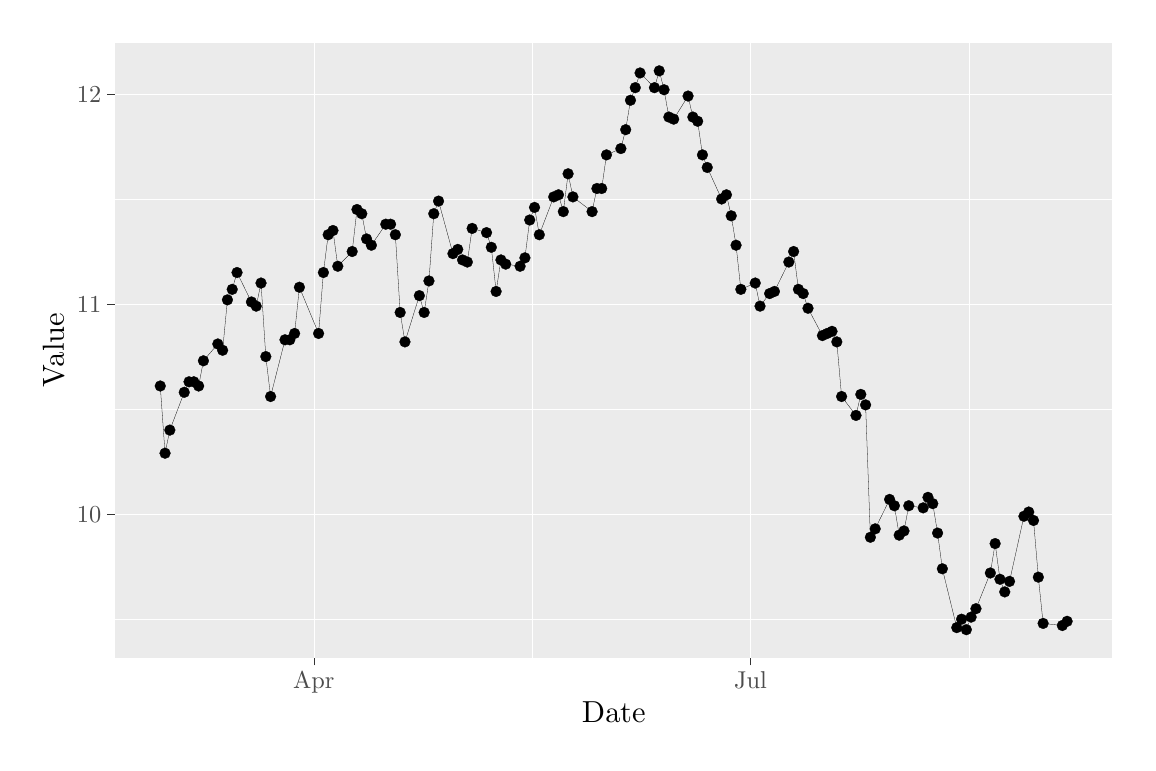
\begin{tikzpicture}[x=1pt,y=1pt]
\definecolor{fillColor}{RGB}{255,255,255}
\path[use as bounding box,fill=fillColor,fill opacity=0.00] (0,0) rectangle (397.48,258.37);
\begin{scope}
\path[clip] (  0.00,  0.00) rectangle (397.48,258.37);
\definecolor{drawColor}{RGB}{255,255,255}
\definecolor{fillColor}{RGB}{255,255,255}

\path[draw=drawColor,line width= 0.1pt,line join=round,line cap=round,fill=fillColor] (  0.00,  0.00) rectangle (397.48,258.37);
\end{scope}
\begin{scope}
\path[clip] ( 31.52, 30.73) rectangle (391.98,252.87);
\definecolor{fillColor}{gray}{0.92}

\path[fill=fillColor] ( 31.52, 30.73) rectangle (391.98,252.87);
\definecolor{drawColor}{RGB}{255,255,255}

\path[draw=drawColor,line width= 0.1pt,line join=round] ( 31.52, 44.62) --
	(391.98, 44.62);

\path[draw=drawColor,line width= 0.1pt,line join=round] ( 31.52,120.54) --
	(391.98,120.54);

\path[draw=drawColor,line width= 0.1pt,line join=round] ( 31.52,196.46) --
	(391.98,196.46);

\path[draw=drawColor,line width= 0.1pt,line join=round] (182.28, 30.73) --
	(182.28,252.87);

\path[draw=drawColor,line width= 0.1pt,line join=round] (340.06, 30.73) --
	(340.06,252.87);

\path[draw=drawColor,line width= 0.1pt,line join=round] ( 31.52, 82.58) --
	(391.98, 82.58);

\path[draw=drawColor,line width= 0.1pt,line join=round] ( 31.52,158.50) --
	(391.98,158.50);

\path[draw=drawColor,line width= 0.1pt,line join=round] ( 31.52,234.42) --
	(391.98,234.42);

\path[draw=drawColor,line width= 0.1pt,line join=round] (103.39, 30.73) --
	(103.39,252.87);

\path[draw=drawColor,line width= 0.1pt,line join=round] (261.17, 30.73) --
	(261.17,252.87);
\definecolor{drawColor}{RGB}{0,0,0}

\path[draw=drawColor,line width= 0.1pt,line join=round] ( 47.91,128.89) --
	( 49.64,104.60) --
	( 51.37,112.95) --
	( 56.58,126.61) --
	( 58.31,130.41) --
	( 60.04,130.41) --
	( 61.78,128.89) --
	( 63.51,138.00) --
	( 68.71,144.07) --
	( 70.45,141.80) --
	( 72.18,160.02) --
	( 73.91,163.81) --
	( 75.65,169.89) --
	( 80.85,159.26) --
	( 82.58,157.74) --
	( 84.32,166.09) --
	( 86.05,139.52) --
	( 87.78,125.09) --
	( 92.99,145.59) --
	( 94.72,145.59) --
	( 96.45,147.87) --
	( 98.19,164.57) --
	(105.12,147.87) --
	(106.86,169.89) --
	(108.59,183.55) --
	(110.32,185.07) --
	(112.06,172.16) --
	(117.26,177.48) --
	(118.99,192.66) --
	(120.73,191.14) --
	(122.46,182.03) --
	(124.20,179.76) --
	(129.40,187.35) --
	(131.13,187.35) --
	(132.86,183.55) --
	(134.60,155.46) --
	(136.33,144.83) --
	(141.53,161.54) --
	(143.27,155.46) --
	(145.00,166.85) --
	(146.74,191.14) --
	(148.47,195.70) --
	(153.67,176.72) --
	(155.40,178.24) --
	(157.14,174.44) --
	(158.87,173.68) --
	(160.61,185.83) --
	(165.81,184.31) --
	(167.54,179.00) --
	(169.27,163.05) --
	(171.01,174.44) --
	(172.74,172.92) --
	(177.94,172.16) --
	(179.68,175.20) --
	(181.41,188.87) --
	(183.15,193.42) --
	(184.88,183.55) --
	(190.08,197.22) --
	(191.81,197.98) --
	(193.55,191.90) --
	(195.28,205.57) --
	(197.02,197.22) --
	(203.95,191.90) --
	(205.69,200.25) --
	(207.42,200.25) --
	(209.15,212.40) --
	(214.35,214.68) --
	(216.09,221.51) --
	(217.82,232.14) --
	(219.56,236.69) --
	(221.29,242.01) --
	(226.49,236.69) --
	(228.22,242.77) --
	(229.96,235.94) --
	(231.69,226.07) --
	(233.43,225.31) --
	(238.63,233.66) --
	(240.36,226.07) --
	(242.10,224.55) --
	(243.83,212.40) --
	(245.56,207.85) --
	(250.76,196.46) --
	(252.50,197.98) --
	(254.23,190.38) --
	(255.97,179.76) --
	(257.70,163.81) --
	(262.90,166.09) --
	(264.64,157.74) --
	(268.10,162.29) --
	(269.84,163.05) --
	(275.04,173.68) --
	(276.77,177.48) --
	(278.51,163.81) --
	(280.24,162.29) --
	(281.97,156.98) --
	(287.18,147.11) --
	(288.91,147.87) --
	(290.64,148.63) --
	(292.38,144.83) --
	(294.11,125.09) --
	(299.31,118.26) --
	(301.05,125.85) --
	(302.78,122.06) --
	(304.51, 74.23) --
	(306.25, 77.27) --
	(311.45, 87.90) --
	(313.18, 85.62) --
	(314.92, 74.99) --
	(316.65, 76.51) --
	(318.38, 85.62) --
	(323.59, 84.86) --
	(325.32, 88.65) --
	(327.05, 86.38) --
	(328.79, 75.75) --
	(330.52, 62.84) --
	(335.72, 41.58) --
	(337.46, 44.62) --
	(339.19, 40.83) --
	(340.92, 45.38) --
	(342.66, 48.42) --
	(347.86, 61.32) --
	(349.59, 71.95) --
	(351.33, 59.05) --
	(353.06, 54.49) --
	(354.79, 58.29) --
	(360.00, 81.82) --
	(361.73, 83.34) --
	(363.46, 80.30) --
	(365.20, 59.81) --
	(366.93, 43.10) --
	(373.87, 42.34) --
	(375.60, 43.86);
\definecolor{fillColor}{RGB}{0,0,0}

\path[draw=drawColor,line width= 0.1pt,line join=round,line cap=round,fill=fillColor] ( 47.91,128.89) circle (  1.96);

\path[draw=drawColor,line width= 0.1pt,line join=round,line cap=round,fill=fillColor] ( 49.64,104.60) circle (  1.96);

\path[draw=drawColor,line width= 0.1pt,line join=round,line cap=round,fill=fillColor] ( 51.37,112.95) circle (  1.96);

\path[draw=drawColor,line width= 0.1pt,line join=round,line cap=round,fill=fillColor] ( 56.58,126.61) circle (  1.96);

\path[draw=drawColor,line width= 0.1pt,line join=round,line cap=round,fill=fillColor] ( 58.31,130.41) circle (  1.96);

\path[draw=drawColor,line width= 0.1pt,line join=round,line cap=round,fill=fillColor] ( 60.04,130.41) circle (  1.96);

\path[draw=drawColor,line width= 0.1pt,line join=round,line cap=round,fill=fillColor] ( 61.78,128.89) circle (  1.96);

\path[draw=drawColor,line width= 0.1pt,line join=round,line cap=round,fill=fillColor] ( 63.51,138.00) circle (  1.96);

\path[draw=drawColor,line width= 0.1pt,line join=round,line cap=round,fill=fillColor] ( 68.71,144.07) circle (  1.96);

\path[draw=drawColor,line width= 0.1pt,line join=round,line cap=round,fill=fillColor] ( 70.45,141.80) circle (  1.96);

\path[draw=drawColor,line width= 0.1pt,line join=round,line cap=round,fill=fillColor] ( 72.18,160.02) circle (  1.96);

\path[draw=drawColor,line width= 0.1pt,line join=round,line cap=round,fill=fillColor] ( 73.91,163.81) circle (  1.96);

\path[draw=drawColor,line width= 0.1pt,line join=round,line cap=round,fill=fillColor] ( 75.65,169.89) circle (  1.96);

\path[draw=drawColor,line width= 0.1pt,line join=round,line cap=round,fill=fillColor] ( 80.85,159.26) circle (  1.96);

\path[draw=drawColor,line width= 0.1pt,line join=round,line cap=round,fill=fillColor] ( 82.58,157.74) circle (  1.96);

\path[draw=drawColor,line width= 0.1pt,line join=round,line cap=round,fill=fillColor] ( 84.32,166.09) circle (  1.96);

\path[draw=drawColor,line width= 0.1pt,line join=round,line cap=round,fill=fillColor] ( 86.05,139.52) circle (  1.96);

\path[draw=drawColor,line width= 0.1pt,line join=round,line cap=round,fill=fillColor] ( 87.78,125.09) circle (  1.96);

\path[draw=drawColor,line width= 0.1pt,line join=round,line cap=round,fill=fillColor] ( 92.99,145.59) circle (  1.96);

\path[draw=drawColor,line width= 0.1pt,line join=round,line cap=round,fill=fillColor] ( 94.72,145.59) circle (  1.96);

\path[draw=drawColor,line width= 0.1pt,line join=round,line cap=round,fill=fillColor] ( 96.45,147.87) circle (  1.96);

\path[draw=drawColor,line width= 0.1pt,line join=round,line cap=round,fill=fillColor] ( 98.19,164.57) circle (  1.96);

\path[draw=drawColor,line width= 0.1pt,line join=round,line cap=round,fill=fillColor] (105.12,147.87) circle (  1.96);

\path[draw=drawColor,line width= 0.1pt,line join=round,line cap=round,fill=fillColor] (106.86,169.89) circle (  1.96);

\path[draw=drawColor,line width= 0.1pt,line join=round,line cap=round,fill=fillColor] (108.59,183.55) circle (  1.96);

\path[draw=drawColor,line width= 0.1pt,line join=round,line cap=round,fill=fillColor] (110.32,185.07) circle (  1.96);

\path[draw=drawColor,line width= 0.1pt,line join=round,line cap=round,fill=fillColor] (112.06,172.16) circle (  1.96);

\path[draw=drawColor,line width= 0.1pt,line join=round,line cap=round,fill=fillColor] (117.26,177.48) circle (  1.96);

\path[draw=drawColor,line width= 0.1pt,line join=round,line cap=round,fill=fillColor] (118.99,192.66) circle (  1.96);

\path[draw=drawColor,line width= 0.1pt,line join=round,line cap=round,fill=fillColor] (120.73,191.14) circle (  1.96);

\path[draw=drawColor,line width= 0.1pt,line join=round,line cap=round,fill=fillColor] (122.46,182.03) circle (  1.96);

\path[draw=drawColor,line width= 0.1pt,line join=round,line cap=round,fill=fillColor] (124.20,179.76) circle (  1.96);

\path[draw=drawColor,line width= 0.1pt,line join=round,line cap=round,fill=fillColor] (129.40,187.35) circle (  1.96);

\path[draw=drawColor,line width= 0.1pt,line join=round,line cap=round,fill=fillColor] (131.13,187.35) circle (  1.96);

\path[draw=drawColor,line width= 0.1pt,line join=round,line cap=round,fill=fillColor] (132.86,183.55) circle (  1.96);

\path[draw=drawColor,line width= 0.1pt,line join=round,line cap=round,fill=fillColor] (134.60,155.46) circle (  1.96);

\path[draw=drawColor,line width= 0.1pt,line join=round,line cap=round,fill=fillColor] (136.33,144.83) circle (  1.96);

\path[draw=drawColor,line width= 0.1pt,line join=round,line cap=round,fill=fillColor] (141.53,161.54) circle (  1.96);

\path[draw=drawColor,line width= 0.1pt,line join=round,line cap=round,fill=fillColor] (143.27,155.46) circle (  1.96);

\path[draw=drawColor,line width= 0.1pt,line join=round,line cap=round,fill=fillColor] (145.00,166.85) circle (  1.96);

\path[draw=drawColor,line width= 0.1pt,line join=round,line cap=round,fill=fillColor] (146.74,191.14) circle (  1.96);

\path[draw=drawColor,line width= 0.1pt,line join=round,line cap=round,fill=fillColor] (148.47,195.70) circle (  1.96);

\path[draw=drawColor,line width= 0.1pt,line join=round,line cap=round,fill=fillColor] (153.67,176.72) circle (  1.96);

\path[draw=drawColor,line width= 0.1pt,line join=round,line cap=round,fill=fillColor] (155.40,178.24) circle (  1.96);

\path[draw=drawColor,line width= 0.1pt,line join=round,line cap=round,fill=fillColor] (157.14,174.44) circle (  1.96);

\path[draw=drawColor,line width= 0.1pt,line join=round,line cap=round,fill=fillColor] (158.87,173.68) circle (  1.96);

\path[draw=drawColor,line width= 0.1pt,line join=round,line cap=round,fill=fillColor] (160.61,185.83) circle (  1.96);

\path[draw=drawColor,line width= 0.1pt,line join=round,line cap=round,fill=fillColor] (165.81,184.31) circle (  1.96);

\path[draw=drawColor,line width= 0.1pt,line join=round,line cap=round,fill=fillColor] (167.54,179.00) circle (  1.96);

\path[draw=drawColor,line width= 0.1pt,line join=round,line cap=round,fill=fillColor] (169.27,163.05) circle (  1.96);

\path[draw=drawColor,line width= 0.1pt,line join=round,line cap=round,fill=fillColor] (171.01,174.44) circle (  1.96);

\path[draw=drawColor,line width= 0.1pt,line join=round,line cap=round,fill=fillColor] (172.74,172.92) circle (  1.96);

\path[draw=drawColor,line width= 0.1pt,line join=round,line cap=round,fill=fillColor] (177.94,172.16) circle (  1.96);

\path[draw=drawColor,line width= 0.1pt,line join=round,line cap=round,fill=fillColor] (179.68,175.20) circle (  1.96);

\path[draw=drawColor,line width= 0.1pt,line join=round,line cap=round,fill=fillColor] (181.41,188.87) circle (  1.96);

\path[draw=drawColor,line width= 0.1pt,line join=round,line cap=round,fill=fillColor] (183.15,193.42) circle (  1.96);

\path[draw=drawColor,line width= 0.1pt,line join=round,line cap=round,fill=fillColor] (184.88,183.55) circle (  1.96);

\path[draw=drawColor,line width= 0.1pt,line join=round,line cap=round,fill=fillColor] (190.08,197.22) circle (  1.96);

\path[draw=drawColor,line width= 0.1pt,line join=round,line cap=round,fill=fillColor] (191.81,197.98) circle (  1.96);

\path[draw=drawColor,line width= 0.1pt,line join=round,line cap=round,fill=fillColor] (193.55,191.90) circle (  1.96);

\path[draw=drawColor,line width= 0.1pt,line join=round,line cap=round,fill=fillColor] (195.28,205.57) circle (  1.96);

\path[draw=drawColor,line width= 0.1pt,line join=round,line cap=round,fill=fillColor] (197.02,197.22) circle (  1.96);

\path[draw=drawColor,line width= 0.1pt,line join=round,line cap=round,fill=fillColor] (203.95,191.90) circle (  1.96);

\path[draw=drawColor,line width= 0.1pt,line join=round,line cap=round,fill=fillColor] (205.69,200.25) circle (  1.96);

\path[draw=drawColor,line width= 0.1pt,line join=round,line cap=round,fill=fillColor] (207.42,200.25) circle (  1.96);

\path[draw=drawColor,line width= 0.1pt,line join=round,line cap=round,fill=fillColor] (209.15,212.40) circle (  1.96);

\path[draw=drawColor,line width= 0.1pt,line join=round,line cap=round,fill=fillColor] (214.35,214.68) circle (  1.96);

\path[draw=drawColor,line width= 0.1pt,line join=round,line cap=round,fill=fillColor] (216.09,221.51) circle (  1.96);

\path[draw=drawColor,line width= 0.1pt,line join=round,line cap=round,fill=fillColor] (217.82,232.14) circle (  1.96);

\path[draw=drawColor,line width= 0.1pt,line join=round,line cap=round,fill=fillColor] (219.56,236.69) circle (  1.96);

\path[draw=drawColor,line width= 0.1pt,line join=round,line cap=round,fill=fillColor] (221.29,242.01) circle (  1.96);

\path[draw=drawColor,line width= 0.1pt,line join=round,line cap=round,fill=fillColor] (226.49,236.69) circle (  1.96);

\path[draw=drawColor,line width= 0.1pt,line join=round,line cap=round,fill=fillColor] (228.22,242.77) circle (  1.96);

\path[draw=drawColor,line width= 0.1pt,line join=round,line cap=round,fill=fillColor] (229.96,235.94) circle (  1.96);

\path[draw=drawColor,line width= 0.1pt,line join=round,line cap=round,fill=fillColor] (231.69,226.07) circle (  1.96);

\path[draw=drawColor,line width= 0.1pt,line join=round,line cap=round,fill=fillColor] (233.43,225.31) circle (  1.96);

\path[draw=drawColor,line width= 0.1pt,line join=round,line cap=round,fill=fillColor] (238.63,233.66) circle (  1.96);

\path[draw=drawColor,line width= 0.1pt,line join=round,line cap=round,fill=fillColor] (240.36,226.07) circle (  1.96);

\path[draw=drawColor,line width= 0.1pt,line join=round,line cap=round,fill=fillColor] (242.10,224.55) circle (  1.96);

\path[draw=drawColor,line width= 0.1pt,line join=round,line cap=round,fill=fillColor] (243.83,212.40) circle (  1.96);

\path[draw=drawColor,line width= 0.1pt,line join=round,line cap=round,fill=fillColor] (245.56,207.85) circle (  1.96);

\path[draw=drawColor,line width= 0.1pt,line join=round,line cap=round,fill=fillColor] (250.76,196.46) circle (  1.96);

\path[draw=drawColor,line width= 0.1pt,line join=round,line cap=round,fill=fillColor] (252.50,197.98) circle (  1.96);

\path[draw=drawColor,line width= 0.1pt,line join=round,line cap=round,fill=fillColor] (254.23,190.38) circle (  1.96);

\path[draw=drawColor,line width= 0.1pt,line join=round,line cap=round,fill=fillColor] (255.97,179.76) circle (  1.96);

\path[draw=drawColor,line width= 0.1pt,line join=round,line cap=round,fill=fillColor] (257.70,163.81) circle (  1.96);

\path[draw=drawColor,line width= 0.1pt,line join=round,line cap=round,fill=fillColor] (262.90,166.09) circle (  1.96);

\path[draw=drawColor,line width= 0.1pt,line join=round,line cap=round,fill=fillColor] (264.64,157.74) circle (  1.96);

\path[draw=drawColor,line width= 0.1pt,line join=round,line cap=round,fill=fillColor] (268.10,162.29) circle (  1.96);

\path[draw=drawColor,line width= 0.1pt,line join=round,line cap=round,fill=fillColor] (269.84,163.05) circle (  1.96);

\path[draw=drawColor,line width= 0.1pt,line join=round,line cap=round,fill=fillColor] (275.04,173.68) circle (  1.96);

\path[draw=drawColor,line width= 0.1pt,line join=round,line cap=round,fill=fillColor] (276.77,177.48) circle (  1.96);

\path[draw=drawColor,line width= 0.1pt,line join=round,line cap=round,fill=fillColor] (278.51,163.81) circle (  1.96);

\path[draw=drawColor,line width= 0.1pt,line join=round,line cap=round,fill=fillColor] (280.24,162.29) circle (  1.96);

\path[draw=drawColor,line width= 0.1pt,line join=round,line cap=round,fill=fillColor] (281.97,156.98) circle (  1.96);

\path[draw=drawColor,line width= 0.1pt,line join=round,line cap=round,fill=fillColor] (287.18,147.11) circle (  1.96);

\path[draw=drawColor,line width= 0.1pt,line join=round,line cap=round,fill=fillColor] (288.91,147.87) circle (  1.96);

\path[draw=drawColor,line width= 0.1pt,line join=round,line cap=round,fill=fillColor] (290.64,148.63) circle (  1.96);

\path[draw=drawColor,line width= 0.1pt,line join=round,line cap=round,fill=fillColor] (292.38,144.83) circle (  1.96);

\path[draw=drawColor,line width= 0.1pt,line join=round,line cap=round,fill=fillColor] (294.11,125.09) circle (  1.96);

\path[draw=drawColor,line width= 0.1pt,line join=round,line cap=round,fill=fillColor] (299.31,118.26) circle (  1.96);

\path[draw=drawColor,line width= 0.1pt,line join=round,line cap=round,fill=fillColor] (301.05,125.85) circle (  1.96);

\path[draw=drawColor,line width= 0.1pt,line join=round,line cap=round,fill=fillColor] (302.78,122.06) circle (  1.96);

\path[draw=drawColor,line width= 0.1pt,line join=round,line cap=round,fill=fillColor] (304.51, 74.23) circle (  1.96);

\path[draw=drawColor,line width= 0.1pt,line join=round,line cap=round,fill=fillColor] (306.25, 77.27) circle (  1.96);

\path[draw=drawColor,line width= 0.1pt,line join=round,line cap=round,fill=fillColor] (311.45, 87.90) circle (  1.96);

\path[draw=drawColor,line width= 0.1pt,line join=round,line cap=round,fill=fillColor] (313.18, 85.62) circle (  1.96);

\path[draw=drawColor,line width= 0.1pt,line join=round,line cap=round,fill=fillColor] (314.92, 74.99) circle (  1.96);

\path[draw=drawColor,line width= 0.1pt,line join=round,line cap=round,fill=fillColor] (316.65, 76.51) circle (  1.96);

\path[draw=drawColor,line width= 0.1pt,line join=round,line cap=round,fill=fillColor] (318.38, 85.62) circle (  1.96);

\path[draw=drawColor,line width= 0.1pt,line join=round,line cap=round,fill=fillColor] (323.59, 84.86) circle (  1.96);

\path[draw=drawColor,line width= 0.1pt,line join=round,line cap=round,fill=fillColor] (325.32, 88.65) circle (  1.96);

\path[draw=drawColor,line width= 0.1pt,line join=round,line cap=round,fill=fillColor] (327.05, 86.38) circle (  1.96);

\path[draw=drawColor,line width= 0.1pt,line join=round,line cap=round,fill=fillColor] (328.79, 75.75) circle (  1.96);

\path[draw=drawColor,line width= 0.1pt,line join=round,line cap=round,fill=fillColor] (330.52, 62.84) circle (  1.96);

\path[draw=drawColor,line width= 0.1pt,line join=round,line cap=round,fill=fillColor] (335.72, 41.58) circle (  1.96);

\path[draw=drawColor,line width= 0.1pt,line join=round,line cap=round,fill=fillColor] (337.46, 44.62) circle (  1.96);

\path[draw=drawColor,line width= 0.1pt,line join=round,line cap=round,fill=fillColor] (339.19, 40.83) circle (  1.96);

\path[draw=drawColor,line width= 0.1pt,line join=round,line cap=round,fill=fillColor] (340.92, 45.38) circle (  1.96);

\path[draw=drawColor,line width= 0.1pt,line join=round,line cap=round,fill=fillColor] (342.66, 48.42) circle (  1.96);

\path[draw=drawColor,line width= 0.1pt,line join=round,line cap=round,fill=fillColor] (347.86, 61.32) circle (  1.96);

\path[draw=drawColor,line width= 0.1pt,line join=round,line cap=round,fill=fillColor] (349.59, 71.95) circle (  1.96);

\path[draw=drawColor,line width= 0.1pt,line join=round,line cap=round,fill=fillColor] (351.33, 59.05) circle (  1.96);

\path[draw=drawColor,line width= 0.1pt,line join=round,line cap=round,fill=fillColor] (353.06, 54.49) circle (  1.96);

\path[draw=drawColor,line width= 0.1pt,line join=round,line cap=round,fill=fillColor] (354.79, 58.29) circle (  1.96);

\path[draw=drawColor,line width= 0.1pt,line join=round,line cap=round,fill=fillColor] (360.00, 81.82) circle (  1.96);

\path[draw=drawColor,line width= 0.1pt,line join=round,line cap=round,fill=fillColor] (361.73, 83.34) circle (  1.96);

\path[draw=drawColor,line width= 0.1pt,line join=round,line cap=round,fill=fillColor] (363.46, 80.30) circle (  1.96);

\path[draw=drawColor,line width= 0.1pt,line join=round,line cap=round,fill=fillColor] (365.20, 59.81) circle (  1.96);

\path[draw=drawColor,line width= 0.1pt,line join=round,line cap=round,fill=fillColor] (366.93, 43.10) circle (  1.96);

\path[draw=drawColor,line width= 0.1pt,line join=round,line cap=round,fill=fillColor] (373.87, 42.34) circle (  1.96);

\path[draw=drawColor,line width= 0.1pt,line join=round,line cap=round,fill=fillColor] (375.60, 43.86) circle (  1.96);
\end{scope}
\begin{scope}
\path[clip] (  0.00,  0.00) rectangle (397.48,258.37);
\definecolor{drawColor}{gray}{0.30}

\node[text=drawColor,anchor=base east,inner sep=0pt, outer sep=0pt, scale=  0.88] at ( 26.57, 79.55) {10};

\node[text=drawColor,anchor=base east,inner sep=0pt, outer sep=0pt, scale=  0.88] at ( 26.57,155.47) {11};

\node[text=drawColor,anchor=base east,inner sep=0pt, outer sep=0pt, scale=  0.88] at ( 26.57,231.39) {12};
\end{scope}
\begin{scope}
\path[clip] (  0.00,  0.00) rectangle (397.48,258.37);
\definecolor{drawColor}{gray}{0.20}

\path[draw=drawColor,line width= 0.1pt,line join=round] ( 28.77, 82.58) --
	( 31.52, 82.58);

\path[draw=drawColor,line width= 0.1pt,line join=round] ( 28.77,158.50) --
	( 31.52,158.50);

\path[draw=drawColor,line width= 0.1pt,line join=round] ( 28.77,234.42) --
	( 31.52,234.42);
\end{scope}
\begin{scope}
\path[clip] (  0.00,  0.00) rectangle (397.48,258.37);
\definecolor{drawColor}{gray}{0.20}

\path[draw=drawColor,line width= 0.1pt,line join=round] (103.39, 27.98) --
	(103.39, 30.73);

\path[draw=drawColor,line width= 0.1pt,line join=round] (261.17, 27.98) --
	(261.17, 30.73);
\end{scope}
\begin{scope}
\path[clip] (  0.00,  0.00) rectangle (397.48,258.37);
\definecolor{drawColor}{gray}{0.30}

\node[text=drawColor,anchor=base,inner sep=0pt, outer sep=0pt, scale=  0.88] at (103.39, 19.72) {Apr};

\node[text=drawColor,anchor=base,inner sep=0pt, outer sep=0pt, scale=  0.88] at (261.17, 19.72) {Jul};
\end{scope}
\begin{scope}
\path[clip] (  0.00,  0.00) rectangle (397.48,258.37);
\definecolor{drawColor}{RGB}{0,0,0}

\node[text=drawColor,anchor=base,inner sep=0pt, outer sep=0pt, scale=  1.10] at (211.75,  7.44) {Date};
\end{scope}
\begin{scope}
\path[clip] (  0.00,  0.00) rectangle (397.48,258.37);
\definecolor{drawColor}{RGB}{0,0,0}

\node[text=drawColor,rotate= 90.00,anchor=base,inner sep=0pt, outer sep=0pt, scale=  1.10] at ( 13.08,141.80) {Value};
\end{scope}
\end{tikzpicture}

    
    \caption{Indices of Ford Motor Company within the evaluation time frame}
    \label{fig:analysis-indices-ford}
\end{figure}    

\subsection{General Motors}
\label{ss:analysis-datasets-gm}

\begin{figure}[hbt]
    \centering
    % Created by tikzDevice version 0.12 on 2019-02-27 16:25:31
% !TEX encoding = UTF-8 Unicode
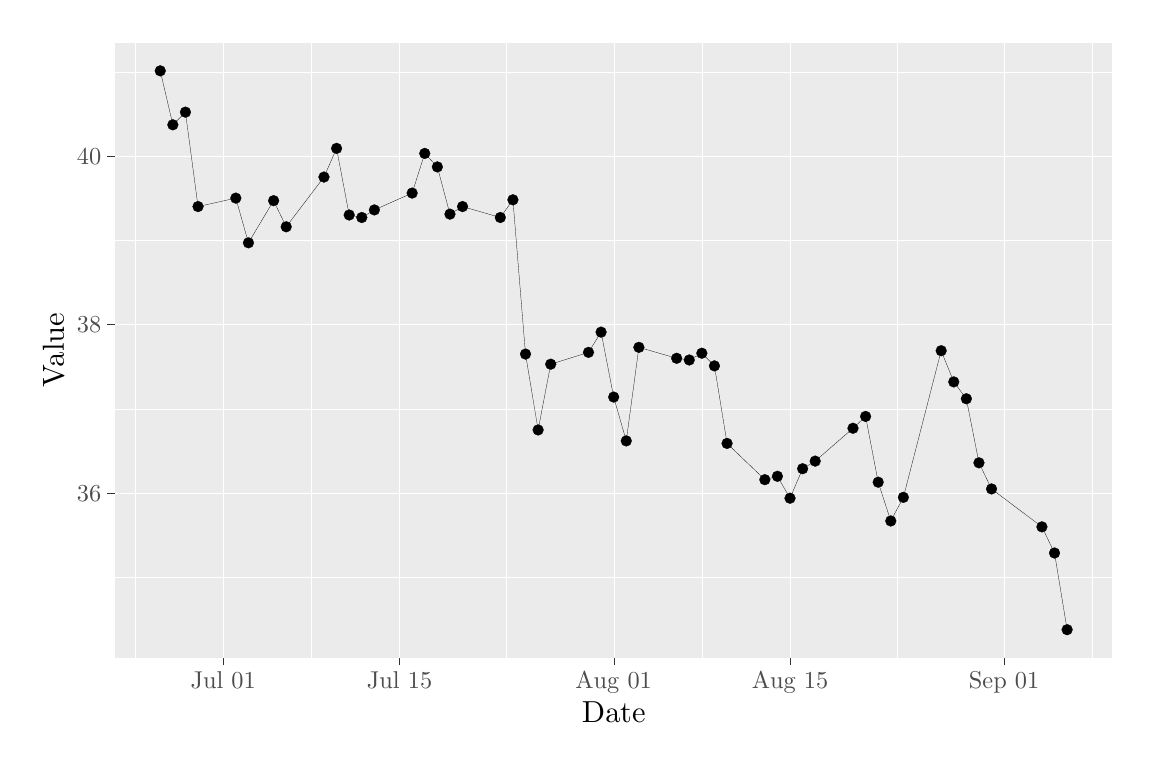
\begin{tikzpicture}[x=1pt,y=1pt]
\definecolor{fillColor}{RGB}{255,255,255}
\path[use as bounding box,fill=fillColor,fill opacity=0.00] (0,0) rectangle (397.48,258.37);
\begin{scope}
\path[clip] (  0.00,  0.00) rectangle (397.48,258.37);
\definecolor{drawColor}{RGB}{255,255,255}
\definecolor{fillColor}{RGB}{255,255,255}

\path[draw=drawColor,line width= 0.1pt,line join=round,line cap=round,fill=fillColor] (  0.00,  0.00) rectangle (397.48,258.37);
\end{scope}
\begin{scope}
\path[clip] ( 31.52, 30.73) rectangle (391.98,252.87);
\definecolor{fillColor}{gray}{0.92}

\path[fill=fillColor] ( 31.52, 30.73) rectangle (391.98,252.87);
\definecolor{drawColor}{RGB}{255,255,255}

\path[draw=drawColor,line width= 0.1pt,line join=round] ( 31.52, 59.71) --
	(391.98, 59.71);

\path[draw=drawColor,line width= 0.1pt,line join=round] ( 31.52,120.63) --
	(391.98,120.63);

\path[draw=drawColor,line width= 0.1pt,line join=round] ( 31.52,181.55) --
	(391.98,181.55);

\path[draw=drawColor,line width= 0.1pt,line join=round] ( 31.52,242.46) --
	(391.98,242.46);

\path[draw=drawColor,line width= 0.1pt,line join=round] ( 38.80, 30.73) --
	( 38.80,252.87);

\path[draw=drawColor,line width= 0.1pt,line join=round] (102.52, 30.73) --
	(102.52,252.87);

\path[draw=drawColor,line width= 0.1pt,line join=round] (173.07, 30.73) --
	(173.07,252.87);

\path[draw=drawColor,line width= 0.1pt,line join=round] (243.61, 30.73) --
	(243.61,252.87);

\path[draw=drawColor,line width= 0.1pt,line join=round] (314.16, 30.73) --
	(314.16,252.87);

\path[draw=drawColor,line width= 0.1pt,line join=round] (384.70, 30.73) --
	(384.70,252.87);

\path[draw=drawColor,line width= 0.1pt,line join=round] ( 31.52, 90.17) --
	(391.98, 90.17);

\path[draw=drawColor,line width= 0.1pt,line join=round] ( 31.52,151.09) --
	(391.98,151.09);

\path[draw=drawColor,line width= 0.1pt,line join=round] ( 31.52,212.00) --
	(391.98,212.00);

\path[draw=drawColor,line width= 0.1pt,line join=round] ( 70.66, 30.73) --
	( 70.66,252.87);

\path[draw=drawColor,line width= 0.1pt,line join=round] (134.38, 30.73) --
	(134.38,252.87);

\path[draw=drawColor,line width= 0.1pt,line join=round] (211.75, 30.73) --
	(211.75,252.87);

\path[draw=drawColor,line width= 0.1pt,line join=round] (275.47, 30.73) --
	(275.47,252.87);

\path[draw=drawColor,line width= 0.1pt,line join=round] (352.84, 30.73) --
	(352.84,252.87);
\definecolor{drawColor}{RGB}{0,0,0}

\path[draw=drawColor,line width= 0.1pt,line join=round] ( 47.91,242.77) --
	( 52.46,223.27) --
	( 57.01,227.84) --
	( 61.56,193.73) --
	( 75.21,196.78) --
	( 79.77,180.63) --
	( 88.87,195.86) --
	( 93.42,186.42) --
	(107.07,204.39) --
	(111.62,214.75) --
	(116.18,190.68) --
	(120.73,189.77) --
	(125.28,192.51) --
	(138.93,198.60) --
	(143.48,212.92) --
	(148.04,208.05) --
	(152.59,190.99) --
	(157.14,193.73) --
	(170.79,189.77) --
	(175.34,196.17) --
	(179.89,140.43) --
	(184.45,113.01) --
	(189.00,136.77) --
	(202.65,141.04) --
	(207.20,148.35) --
	(211.75,124.89) --
	(216.30,109.05) --
	(220.86,142.86) --
	(234.51,138.90) --
	(239.06,138.29) --
	(243.61,140.73) --
	(248.16,136.16) --
	(252.72,108.14) --
	(266.37, 95.04) --
	(270.92, 96.26) --
	(275.47, 88.34) --
	(280.02, 99.00) --
	(284.57,101.74) --
	(298.23,113.62) --
	(302.78,117.89) --
	(307.33, 94.13) --
	(311.88, 80.12) --
	(316.43, 88.65) --
	(330.09,141.64) --
	(334.64,130.37) --
	(339.19,124.28) --
	(343.74,101.13) --
	(348.29, 91.69) --
	(366.50, 77.99) --
	(371.05, 68.54) --
	(375.60, 40.83);
\definecolor{fillColor}{RGB}{0,0,0}

\path[draw=drawColor,line width= 0.1pt,line join=round,line cap=round,fill=fillColor] ( 47.91,242.77) circle (  1.96);

\path[draw=drawColor,line width= 0.1pt,line join=round,line cap=round,fill=fillColor] ( 52.46,223.27) circle (  1.96);

\path[draw=drawColor,line width= 0.1pt,line join=round,line cap=round,fill=fillColor] ( 57.01,227.84) circle (  1.96);

\path[draw=drawColor,line width= 0.1pt,line join=round,line cap=round,fill=fillColor] ( 61.56,193.73) circle (  1.96);

\path[draw=drawColor,line width= 0.1pt,line join=round,line cap=round,fill=fillColor] ( 75.21,196.78) circle (  1.96);

\path[draw=drawColor,line width= 0.1pt,line join=round,line cap=round,fill=fillColor] ( 79.77,180.63) circle (  1.96);

\path[draw=drawColor,line width= 0.1pt,line join=round,line cap=round,fill=fillColor] ( 88.87,195.86) circle (  1.96);

\path[draw=drawColor,line width= 0.1pt,line join=round,line cap=round,fill=fillColor] ( 93.42,186.42) circle (  1.96);

\path[draw=drawColor,line width= 0.1pt,line join=round,line cap=round,fill=fillColor] (107.07,204.39) circle (  1.96);

\path[draw=drawColor,line width= 0.1pt,line join=round,line cap=round,fill=fillColor] (111.62,214.75) circle (  1.96);

\path[draw=drawColor,line width= 0.1pt,line join=round,line cap=round,fill=fillColor] (116.18,190.68) circle (  1.96);

\path[draw=drawColor,line width= 0.1pt,line join=round,line cap=round,fill=fillColor] (120.73,189.77) circle (  1.96);

\path[draw=drawColor,line width= 0.1pt,line join=round,line cap=round,fill=fillColor] (125.28,192.51) circle (  1.96);

\path[draw=drawColor,line width= 0.1pt,line join=round,line cap=round,fill=fillColor] (138.93,198.60) circle (  1.96);

\path[draw=drawColor,line width= 0.1pt,line join=round,line cap=round,fill=fillColor] (143.48,212.92) circle (  1.96);

\path[draw=drawColor,line width= 0.1pt,line join=round,line cap=round,fill=fillColor] (148.04,208.05) circle (  1.96);

\path[draw=drawColor,line width= 0.1pt,line join=round,line cap=round,fill=fillColor] (152.59,190.99) circle (  1.96);

\path[draw=drawColor,line width= 0.1pt,line join=round,line cap=round,fill=fillColor] (157.14,193.73) circle (  1.96);

\path[draw=drawColor,line width= 0.1pt,line join=round,line cap=round,fill=fillColor] (170.79,189.77) circle (  1.96);

\path[draw=drawColor,line width= 0.1pt,line join=round,line cap=round,fill=fillColor] (175.34,196.17) circle (  1.96);

\path[draw=drawColor,line width= 0.1pt,line join=round,line cap=round,fill=fillColor] (179.89,140.43) circle (  1.96);

\path[draw=drawColor,line width= 0.1pt,line join=round,line cap=round,fill=fillColor] (184.45,113.01) circle (  1.96);

\path[draw=drawColor,line width= 0.1pt,line join=round,line cap=round,fill=fillColor] (189.00,136.77) circle (  1.96);

\path[draw=drawColor,line width= 0.1pt,line join=round,line cap=round,fill=fillColor] (202.65,141.04) circle (  1.96);

\path[draw=drawColor,line width= 0.1pt,line join=round,line cap=round,fill=fillColor] (207.20,148.35) circle (  1.96);

\path[draw=drawColor,line width= 0.1pt,line join=round,line cap=round,fill=fillColor] (211.75,124.89) circle (  1.96);

\path[draw=drawColor,line width= 0.1pt,line join=round,line cap=round,fill=fillColor] (216.30,109.05) circle (  1.96);

\path[draw=drawColor,line width= 0.1pt,line join=round,line cap=round,fill=fillColor] (220.86,142.86) circle (  1.96);

\path[draw=drawColor,line width= 0.1pt,line join=round,line cap=round,fill=fillColor] (234.51,138.90) circle (  1.96);

\path[draw=drawColor,line width= 0.1pt,line join=round,line cap=round,fill=fillColor] (239.06,138.29) circle (  1.96);

\path[draw=drawColor,line width= 0.1pt,line join=round,line cap=round,fill=fillColor] (243.61,140.73) circle (  1.96);

\path[draw=drawColor,line width= 0.1pt,line join=round,line cap=round,fill=fillColor] (248.16,136.16) circle (  1.96);

\path[draw=drawColor,line width= 0.1pt,line join=round,line cap=round,fill=fillColor] (252.72,108.14) circle (  1.96);

\path[draw=drawColor,line width= 0.1pt,line join=round,line cap=round,fill=fillColor] (266.37, 95.04) circle (  1.96);

\path[draw=drawColor,line width= 0.1pt,line join=round,line cap=round,fill=fillColor] (270.92, 96.26) circle (  1.96);

\path[draw=drawColor,line width= 0.1pt,line join=round,line cap=round,fill=fillColor] (275.47, 88.34) circle (  1.96);

\path[draw=drawColor,line width= 0.1pt,line join=round,line cap=round,fill=fillColor] (280.02, 99.00) circle (  1.96);

\path[draw=drawColor,line width= 0.1pt,line join=round,line cap=round,fill=fillColor] (284.57,101.74) circle (  1.96);

\path[draw=drawColor,line width= 0.1pt,line join=round,line cap=round,fill=fillColor] (298.23,113.62) circle (  1.96);

\path[draw=drawColor,line width= 0.1pt,line join=round,line cap=round,fill=fillColor] (302.78,117.89) circle (  1.96);

\path[draw=drawColor,line width= 0.1pt,line join=round,line cap=round,fill=fillColor] (307.33, 94.13) circle (  1.96);

\path[draw=drawColor,line width= 0.1pt,line join=round,line cap=round,fill=fillColor] (311.88, 80.12) circle (  1.96);

\path[draw=drawColor,line width= 0.1pt,line join=round,line cap=round,fill=fillColor] (316.43, 88.65) circle (  1.96);

\path[draw=drawColor,line width= 0.1pt,line join=round,line cap=round,fill=fillColor] (330.09,141.64) circle (  1.96);

\path[draw=drawColor,line width= 0.1pt,line join=round,line cap=round,fill=fillColor] (334.64,130.37) circle (  1.96);

\path[draw=drawColor,line width= 0.1pt,line join=round,line cap=round,fill=fillColor] (339.19,124.28) circle (  1.96);

\path[draw=drawColor,line width= 0.1pt,line join=round,line cap=round,fill=fillColor] (343.74,101.13) circle (  1.96);

\path[draw=drawColor,line width= 0.1pt,line join=round,line cap=round,fill=fillColor] (348.29, 91.69) circle (  1.96);

\path[draw=drawColor,line width= 0.1pt,line join=round,line cap=round,fill=fillColor] (366.50, 77.99) circle (  1.96);

\path[draw=drawColor,line width= 0.1pt,line join=round,line cap=round,fill=fillColor] (371.05, 68.54) circle (  1.96);

\path[draw=drawColor,line width= 0.1pt,line join=round,line cap=round,fill=fillColor] (375.60, 40.83) circle (  1.96);
\end{scope}
\begin{scope}
\path[clip] (  0.00,  0.00) rectangle (397.48,258.37);
\definecolor{drawColor}{gray}{0.30}

\node[text=drawColor,anchor=base east,inner sep=0pt, outer sep=0pt, scale=  0.88] at ( 26.57, 87.14) {36};

\node[text=drawColor,anchor=base east,inner sep=0pt, outer sep=0pt, scale=  0.88] at ( 26.57,148.06) {38};

\node[text=drawColor,anchor=base east,inner sep=0pt, outer sep=0pt, scale=  0.88] at ( 26.57,208.97) {40};
\end{scope}
\begin{scope}
\path[clip] (  0.00,  0.00) rectangle (397.48,258.37);
\definecolor{drawColor}{gray}{0.20}

\path[draw=drawColor,line width= 0.1pt,line join=round] ( 28.77, 90.17) --
	( 31.52, 90.17);

\path[draw=drawColor,line width= 0.1pt,line join=round] ( 28.77,151.09) --
	( 31.52,151.09);

\path[draw=drawColor,line width= 0.1pt,line join=round] ( 28.77,212.00) --
	( 31.52,212.00);
\end{scope}
\begin{scope}
\path[clip] (  0.00,  0.00) rectangle (397.48,258.37);
\definecolor{drawColor}{gray}{0.20}

\path[draw=drawColor,line width= 0.1pt,line join=round] ( 70.66, 27.98) --
	( 70.66, 30.73);

\path[draw=drawColor,line width= 0.1pt,line join=round] (134.38, 27.98) --
	(134.38, 30.73);

\path[draw=drawColor,line width= 0.1pt,line join=round] (211.75, 27.98) --
	(211.75, 30.73);

\path[draw=drawColor,line width= 0.1pt,line join=round] (275.47, 27.98) --
	(275.47, 30.73);

\path[draw=drawColor,line width= 0.1pt,line join=round] (352.84, 27.98) --
	(352.84, 30.73);
\end{scope}
\begin{scope}
\path[clip] (  0.00,  0.00) rectangle (397.48,258.37);
\definecolor{drawColor}{gray}{0.30}

\node[text=drawColor,anchor=base,inner sep=0pt, outer sep=0pt, scale=  0.88] at ( 70.66, 19.72) {Jul 01};

\node[text=drawColor,anchor=base,inner sep=0pt, outer sep=0pt, scale=  0.88] at (134.38, 19.72) {Jul 15};

\node[text=drawColor,anchor=base,inner sep=0pt, outer sep=0pt, scale=  0.88] at (211.75, 19.72) {Aug 01};

\node[text=drawColor,anchor=base,inner sep=0pt, outer sep=0pt, scale=  0.88] at (275.47, 19.72) {Aug 15};

\node[text=drawColor,anchor=base,inner sep=0pt, outer sep=0pt, scale=  0.88] at (352.84, 19.72) {Sep 01};
\end{scope}
\begin{scope}
\path[clip] (  0.00,  0.00) rectangle (397.48,258.37);
\definecolor{drawColor}{RGB}{0,0,0}

\node[text=drawColor,anchor=base,inner sep=0pt, outer sep=0pt, scale=  1.10] at (211.75,  7.44) {Date};
\end{scope}
\begin{scope}
\path[clip] (  0.00,  0.00) rectangle (397.48,258.37);
\definecolor{drawColor}{RGB}{0,0,0}

\node[text=drawColor,rotate= 90.00,anchor=base,inner sep=0pt, outer sep=0pt, scale=  1.10] at ( 13.08,141.80) {Value};
\end{scope}
\end{tikzpicture}

    
    \caption{Indices of General Motors within the evaluation time frame}
    \label{fig:analysis-indices-gm}
\end{figure}   

\subsection{Hyundai}
\label{ss:analysis-datasets-hyundai}

\begin{figure}[hbt]
    \centering
    % Created by tikzDevice version 0.12 on 2019-02-27 16:25:30
% !TEX encoding = UTF-8 Unicode
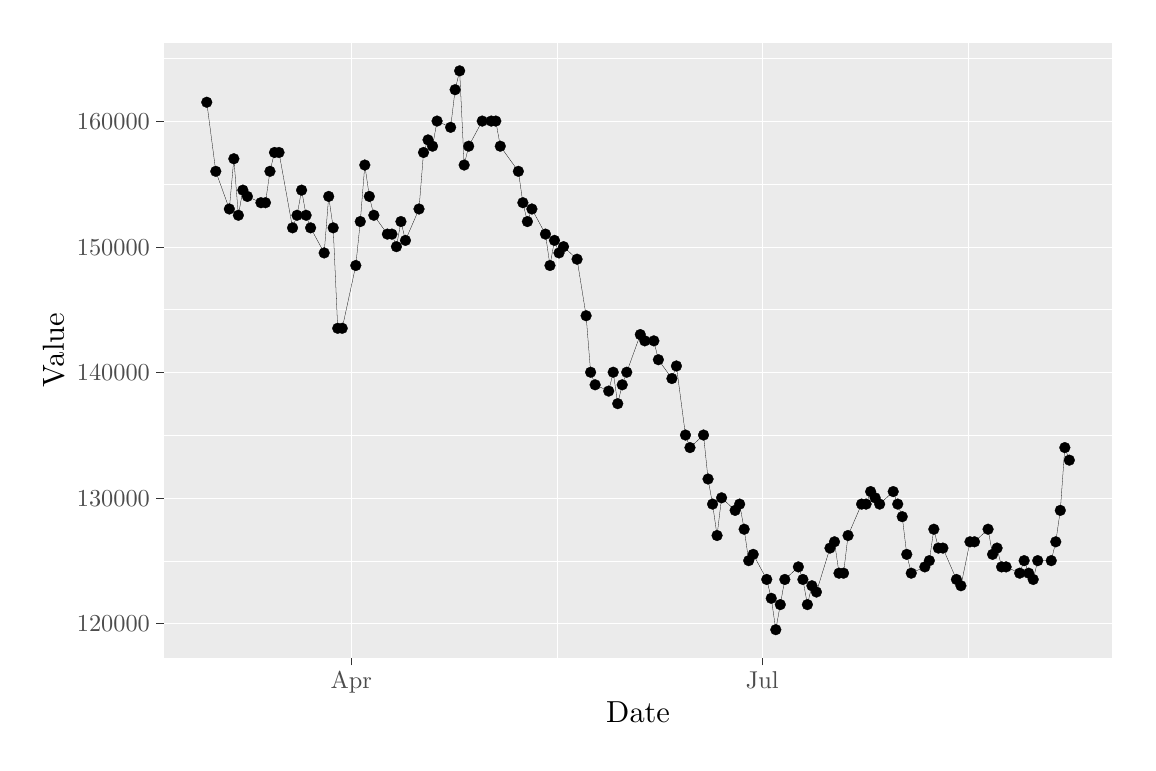
\begin{tikzpicture}[x=1pt,y=1pt]
\definecolor{fillColor}{RGB}{255,255,255}
\path[use as bounding box,fill=fillColor,fill opacity=0.00] (0,0) rectangle (397.48,258.37);
\begin{scope}
\path[clip] (  0.00,  0.00) rectangle (397.48,258.37);
\definecolor{drawColor}{RGB}{255,255,255}
\definecolor{fillColor}{RGB}{255,255,255}

\path[draw=drawColor,line width= 0.1pt,line join=round,line cap=round,fill=fillColor] (  0.00,  0.00) rectangle (397.48,258.37);
\end{scope}
\begin{scope}
\path[clip] ( 49.12, 30.73) rectangle (391.98,252.87);
\definecolor{fillColor}{gray}{0.92}

\path[fill=fillColor] ( 49.12, 30.73) rectangle (391.98,252.87);
\definecolor{drawColor}{RGB}{255,255,255}

\path[draw=drawColor,line width= 0.1pt,line join=round] ( 49.12, 65.78) --
	(391.98, 65.78);

\path[draw=drawColor,line width= 0.1pt,line join=round] ( 49.12,111.17) --
	(391.98,111.17);

\path[draw=drawColor,line width= 0.1pt,line join=round] ( 49.12,156.55) --
	(391.98,156.55);

\path[draw=drawColor,line width= 0.1pt,line join=round] ( 49.12,201.93) --
	(391.98,201.93);

\path[draw=drawColor,line width= 0.1pt,line join=round] ( 49.12,247.31) --
	(391.98,247.31);

\path[draw=drawColor,line width= 0.1pt,line join=round] (191.18, 30.73) --
	(191.18,252.87);

\path[draw=drawColor,line width= 0.1pt,line join=round] (339.68, 30.73) --
	(339.68,252.87);

\path[draw=drawColor,line width= 0.1pt,line join=round] ( 49.12, 43.09) --
	(391.98, 43.09);

\path[draw=drawColor,line width= 0.1pt,line join=round] ( 49.12, 88.48) --
	(391.98, 88.48);

\path[draw=drawColor,line width= 0.1pt,line join=round] ( 49.12,133.86) --
	(391.98,133.86);

\path[draw=drawColor,line width= 0.1pt,line join=round] ( 49.12,179.24) --
	(391.98,179.24);

\path[draw=drawColor,line width= 0.1pt,line join=round] ( 49.12,224.62) --
	(391.98,224.62);

\path[draw=drawColor,line width= 0.1pt,line join=round] (116.93, 30.73) --
	(116.93,252.87);

\path[draw=drawColor,line width= 0.1pt,line join=round] (265.43, 30.73) --
	(265.43,252.87);
\definecolor{drawColor}{RGB}{0,0,0}

\path[draw=drawColor,line width= 0.1pt,line join=round] ( 64.71,231.42) --
	( 67.97,206.46) --
	( 72.87,192.85) --
	( 74.50,211.00) --
	( 76.13,190.58) --
	( 77.76,199.66) --
	( 79.39,197.39) --
	( 84.29,195.12) --
	( 85.92,195.12) --
	( 87.55,206.46) --
	( 89.19,213.27) --
	( 90.82,213.27) --
	( 95.71,186.04) --
	( 97.34,190.58) --
	( 98.98,199.66) --
	(100.61,190.58) --
	(102.24,186.04) --
	(107.14,176.97) --
	(108.77,197.39) --
	(110.40,186.04) --
	(112.03,149.74) --
	(113.66,149.74) --
	(118.56,172.43) --
	(120.19,188.31) --
	(121.82,208.73) --
	(123.46,197.39) --
	(125.09,190.58) --
	(129.98,183.77) --
	(131.61,183.77) --
	(133.25,179.24) --
	(134.88,188.31) --
	(136.51,181.50) --
	(141.41,192.85) --
	(143.04,213.27) --
	(144.67,217.81) --
	(146.30,215.54) --
	(147.93,224.62) --
	(152.83,222.35) --
	(154.46,235.96) --
	(156.09,242.77) --
	(157.73,208.73) --
	(159.36,215.54) --
	(164.25,224.62) --
	(167.52,224.62) --
	(169.15,224.62) --
	(170.78,215.54) --
	(177.31,206.46) --
	(178.94,195.12) --
	(180.57,188.31) --
	(182.20,192.85) --
	(187.10,183.77) --
	(188.73,172.43) --
	(190.36,181.50) --
	(192.00,176.97) --
	(193.63,179.24) --
	(198.52,174.70) --
	(201.79,154.28) --
	(203.42,133.86) --
	(205.05,129.32) --
	(209.95,127.05) --
	(211.58,133.86) --
	(213.21,122.51) --
	(214.84,129.32) --
	(216.47,133.86) --
	(221.37,147.47) --
	(223.00,145.20) --
	(226.27,145.20) --
	(227.90,138.39) --
	(232.79,131.59) --
	(234.42,136.12) --
	(237.69,111.17) --
	(239.32,106.63) --
	(244.22,111.17) --
	(245.85, 95.28) --
	(247.48, 86.21) --
	(249.11, 74.86) --
	(250.74, 88.48) --
	(255.64, 83.94) --
	(257.27, 86.21) --
	(258.90, 77.13) --
	(260.54, 65.78) --
	(262.17, 68.05) --
	(267.06, 58.98) --
	(268.69, 52.17) --
	(270.33, 40.83) --
	(271.96, 49.90) --
	(273.59, 58.98) --
	(278.49, 63.52) --
	(280.12, 58.98) --
	(281.75, 49.90) --
	(283.38, 56.71) --
	(285.01, 54.44) --
	(289.91, 70.32) --
	(291.54, 72.59) --
	(293.17, 61.25) --
	(294.81, 61.25) --
	(296.44, 74.86) --
	(301.33, 86.21) --
	(302.96, 86.21) --
	(304.60, 90.74) --
	(306.23, 88.48) --
	(307.86, 86.21) --
	(312.76, 90.74) --
	(314.39, 86.21) --
	(316.02, 81.67) --
	(317.65, 68.05) --
	(319.28, 61.25) --
	(324.18, 63.52) --
	(325.81, 65.78) --
	(327.44, 77.13) --
	(329.08, 70.32) --
	(330.71, 70.32) --
	(335.60, 58.98) --
	(337.23, 56.71) --
	(340.50, 72.59) --
	(342.13, 72.59) --
	(347.03, 77.13) --
	(348.66, 68.05) --
	(350.29, 70.32) --
	(351.92, 63.52) --
	(353.55, 63.52) --
	(358.45, 61.25) --
	(360.08, 65.78) --
	(361.71, 61.25) --
	(363.35, 58.98) --
	(364.98, 65.78) --
	(369.87, 65.78) --
	(371.50, 72.59) --
	(373.14, 83.94) --
	(374.77,106.63) --
	(376.40,102.09);
\definecolor{fillColor}{RGB}{0,0,0}

\path[draw=drawColor,line width= 0.1pt,line join=round,line cap=round,fill=fillColor] ( 64.71,231.42) circle (  1.96);

\path[draw=drawColor,line width= 0.1pt,line join=round,line cap=round,fill=fillColor] ( 67.97,206.46) circle (  1.96);

\path[draw=drawColor,line width= 0.1pt,line join=round,line cap=round,fill=fillColor] ( 72.87,192.85) circle (  1.96);

\path[draw=drawColor,line width= 0.1pt,line join=round,line cap=round,fill=fillColor] ( 74.50,211.00) circle (  1.96);

\path[draw=drawColor,line width= 0.1pt,line join=round,line cap=round,fill=fillColor] ( 76.13,190.58) circle (  1.96);

\path[draw=drawColor,line width= 0.1pt,line join=round,line cap=round,fill=fillColor] ( 77.76,199.66) circle (  1.96);

\path[draw=drawColor,line width= 0.1pt,line join=round,line cap=round,fill=fillColor] ( 79.39,197.39) circle (  1.96);

\path[draw=drawColor,line width= 0.1pt,line join=round,line cap=round,fill=fillColor] ( 84.29,195.12) circle (  1.96);

\path[draw=drawColor,line width= 0.1pt,line join=round,line cap=round,fill=fillColor] ( 85.92,195.12) circle (  1.96);

\path[draw=drawColor,line width= 0.1pt,line join=round,line cap=round,fill=fillColor] ( 87.55,206.46) circle (  1.96);

\path[draw=drawColor,line width= 0.1pt,line join=round,line cap=round,fill=fillColor] ( 89.19,213.27) circle (  1.96);

\path[draw=drawColor,line width= 0.1pt,line join=round,line cap=round,fill=fillColor] ( 90.82,213.27) circle (  1.96);

\path[draw=drawColor,line width= 0.1pt,line join=round,line cap=round,fill=fillColor] ( 95.71,186.04) circle (  1.96);

\path[draw=drawColor,line width= 0.1pt,line join=round,line cap=round,fill=fillColor] ( 97.34,190.58) circle (  1.96);

\path[draw=drawColor,line width= 0.1pt,line join=round,line cap=round,fill=fillColor] ( 98.98,199.66) circle (  1.96);

\path[draw=drawColor,line width= 0.1pt,line join=round,line cap=round,fill=fillColor] (100.61,190.58) circle (  1.96);

\path[draw=drawColor,line width= 0.1pt,line join=round,line cap=round,fill=fillColor] (102.24,186.04) circle (  1.96);

\path[draw=drawColor,line width= 0.1pt,line join=round,line cap=round,fill=fillColor] (107.14,176.97) circle (  1.96);

\path[draw=drawColor,line width= 0.1pt,line join=round,line cap=round,fill=fillColor] (108.77,197.39) circle (  1.96);

\path[draw=drawColor,line width= 0.1pt,line join=round,line cap=round,fill=fillColor] (110.40,186.04) circle (  1.96);

\path[draw=drawColor,line width= 0.1pt,line join=round,line cap=round,fill=fillColor] (112.03,149.74) circle (  1.96);

\path[draw=drawColor,line width= 0.1pt,line join=round,line cap=round,fill=fillColor] (113.66,149.74) circle (  1.96);

\path[draw=drawColor,line width= 0.1pt,line join=round,line cap=round,fill=fillColor] (118.56,172.43) circle (  1.96);

\path[draw=drawColor,line width= 0.1pt,line join=round,line cap=round,fill=fillColor] (120.19,188.31) circle (  1.96);

\path[draw=drawColor,line width= 0.1pt,line join=round,line cap=round,fill=fillColor] (121.82,208.73) circle (  1.96);

\path[draw=drawColor,line width= 0.1pt,line join=round,line cap=round,fill=fillColor] (123.46,197.39) circle (  1.96);

\path[draw=drawColor,line width= 0.1pt,line join=round,line cap=round,fill=fillColor] (125.09,190.58) circle (  1.96);

\path[draw=drawColor,line width= 0.1pt,line join=round,line cap=round,fill=fillColor] (129.98,183.77) circle (  1.96);

\path[draw=drawColor,line width= 0.1pt,line join=round,line cap=round,fill=fillColor] (131.61,183.77) circle (  1.96);

\path[draw=drawColor,line width= 0.1pt,line join=round,line cap=round,fill=fillColor] (133.25,179.24) circle (  1.96);

\path[draw=drawColor,line width= 0.1pt,line join=round,line cap=round,fill=fillColor] (134.88,188.31) circle (  1.96);

\path[draw=drawColor,line width= 0.1pt,line join=round,line cap=round,fill=fillColor] (136.51,181.50) circle (  1.96);

\path[draw=drawColor,line width= 0.1pt,line join=round,line cap=round,fill=fillColor] (141.41,192.85) circle (  1.96);

\path[draw=drawColor,line width= 0.1pt,line join=round,line cap=round,fill=fillColor] (143.04,213.27) circle (  1.96);

\path[draw=drawColor,line width= 0.1pt,line join=round,line cap=round,fill=fillColor] (144.67,217.81) circle (  1.96);

\path[draw=drawColor,line width= 0.1pt,line join=round,line cap=round,fill=fillColor] (146.30,215.54) circle (  1.96);

\path[draw=drawColor,line width= 0.1pt,line join=round,line cap=round,fill=fillColor] (147.93,224.62) circle (  1.96);

\path[draw=drawColor,line width= 0.1pt,line join=round,line cap=round,fill=fillColor] (152.83,222.35) circle (  1.96);

\path[draw=drawColor,line width= 0.1pt,line join=round,line cap=round,fill=fillColor] (154.46,235.96) circle (  1.96);

\path[draw=drawColor,line width= 0.1pt,line join=round,line cap=round,fill=fillColor] (156.09,242.77) circle (  1.96);

\path[draw=drawColor,line width= 0.1pt,line join=round,line cap=round,fill=fillColor] (157.73,208.73) circle (  1.96);

\path[draw=drawColor,line width= 0.1pt,line join=round,line cap=round,fill=fillColor] (159.36,215.54) circle (  1.96);

\path[draw=drawColor,line width= 0.1pt,line join=round,line cap=round,fill=fillColor] (164.25,224.62) circle (  1.96);

\path[draw=drawColor,line width= 0.1pt,line join=round,line cap=round,fill=fillColor] (167.52,224.62) circle (  1.96);

\path[draw=drawColor,line width= 0.1pt,line join=round,line cap=round,fill=fillColor] (169.15,224.62) circle (  1.96);

\path[draw=drawColor,line width= 0.1pt,line join=round,line cap=round,fill=fillColor] (170.78,215.54) circle (  1.96);

\path[draw=drawColor,line width= 0.1pt,line join=round,line cap=round,fill=fillColor] (177.31,206.46) circle (  1.96);

\path[draw=drawColor,line width= 0.1pt,line join=round,line cap=round,fill=fillColor] (178.94,195.12) circle (  1.96);

\path[draw=drawColor,line width= 0.1pt,line join=round,line cap=round,fill=fillColor] (180.57,188.31) circle (  1.96);

\path[draw=drawColor,line width= 0.1pt,line join=round,line cap=round,fill=fillColor] (182.20,192.85) circle (  1.96);

\path[draw=drawColor,line width= 0.1pt,line join=round,line cap=round,fill=fillColor] (187.10,183.77) circle (  1.96);

\path[draw=drawColor,line width= 0.1pt,line join=round,line cap=round,fill=fillColor] (188.73,172.43) circle (  1.96);

\path[draw=drawColor,line width= 0.1pt,line join=round,line cap=round,fill=fillColor] (190.36,181.50) circle (  1.96);

\path[draw=drawColor,line width= 0.1pt,line join=round,line cap=round,fill=fillColor] (192.00,176.97) circle (  1.96);

\path[draw=drawColor,line width= 0.1pt,line join=round,line cap=round,fill=fillColor] (193.63,179.24) circle (  1.96);

\path[draw=drawColor,line width= 0.1pt,line join=round,line cap=round,fill=fillColor] (198.52,174.70) circle (  1.96);

\path[draw=drawColor,line width= 0.1pt,line join=round,line cap=round,fill=fillColor] (201.79,154.28) circle (  1.96);

\path[draw=drawColor,line width= 0.1pt,line join=round,line cap=round,fill=fillColor] (203.42,133.86) circle (  1.96);

\path[draw=drawColor,line width= 0.1pt,line join=round,line cap=round,fill=fillColor] (205.05,129.32) circle (  1.96);

\path[draw=drawColor,line width= 0.1pt,line join=round,line cap=round,fill=fillColor] (209.95,127.05) circle (  1.96);

\path[draw=drawColor,line width= 0.1pt,line join=round,line cap=round,fill=fillColor] (211.58,133.86) circle (  1.96);

\path[draw=drawColor,line width= 0.1pt,line join=round,line cap=round,fill=fillColor] (213.21,122.51) circle (  1.96);

\path[draw=drawColor,line width= 0.1pt,line join=round,line cap=round,fill=fillColor] (214.84,129.32) circle (  1.96);

\path[draw=drawColor,line width= 0.1pt,line join=round,line cap=round,fill=fillColor] (216.47,133.86) circle (  1.96);

\path[draw=drawColor,line width= 0.1pt,line join=round,line cap=round,fill=fillColor] (221.37,147.47) circle (  1.96);

\path[draw=drawColor,line width= 0.1pt,line join=round,line cap=round,fill=fillColor] (223.00,145.20) circle (  1.96);

\path[draw=drawColor,line width= 0.1pt,line join=round,line cap=round,fill=fillColor] (226.27,145.20) circle (  1.96);

\path[draw=drawColor,line width= 0.1pt,line join=round,line cap=round,fill=fillColor] (227.90,138.39) circle (  1.96);

\path[draw=drawColor,line width= 0.1pt,line join=round,line cap=round,fill=fillColor] (232.79,131.59) circle (  1.96);

\path[draw=drawColor,line width= 0.1pt,line join=round,line cap=round,fill=fillColor] (234.42,136.12) circle (  1.96);

\path[draw=drawColor,line width= 0.1pt,line join=round,line cap=round,fill=fillColor] (237.69,111.17) circle (  1.96);

\path[draw=drawColor,line width= 0.1pt,line join=round,line cap=round,fill=fillColor] (239.32,106.63) circle (  1.96);

\path[draw=drawColor,line width= 0.1pt,line join=round,line cap=round,fill=fillColor] (244.22,111.17) circle (  1.96);

\path[draw=drawColor,line width= 0.1pt,line join=round,line cap=round,fill=fillColor] (245.85, 95.28) circle (  1.96);

\path[draw=drawColor,line width= 0.1pt,line join=round,line cap=round,fill=fillColor] (247.48, 86.21) circle (  1.96);

\path[draw=drawColor,line width= 0.1pt,line join=round,line cap=round,fill=fillColor] (249.11, 74.86) circle (  1.96);

\path[draw=drawColor,line width= 0.1pt,line join=round,line cap=round,fill=fillColor] (250.74, 88.48) circle (  1.96);

\path[draw=drawColor,line width= 0.1pt,line join=round,line cap=round,fill=fillColor] (255.64, 83.94) circle (  1.96);

\path[draw=drawColor,line width= 0.1pt,line join=round,line cap=round,fill=fillColor] (257.27, 86.21) circle (  1.96);

\path[draw=drawColor,line width= 0.1pt,line join=round,line cap=round,fill=fillColor] (258.90, 77.13) circle (  1.96);

\path[draw=drawColor,line width= 0.1pt,line join=round,line cap=round,fill=fillColor] (260.54, 65.78) circle (  1.96);

\path[draw=drawColor,line width= 0.1pt,line join=round,line cap=round,fill=fillColor] (262.17, 68.05) circle (  1.96);

\path[draw=drawColor,line width= 0.1pt,line join=round,line cap=round,fill=fillColor] (267.06, 58.98) circle (  1.96);

\path[draw=drawColor,line width= 0.1pt,line join=round,line cap=round,fill=fillColor] (268.69, 52.17) circle (  1.96);

\path[draw=drawColor,line width= 0.1pt,line join=round,line cap=round,fill=fillColor] (270.33, 40.83) circle (  1.96);

\path[draw=drawColor,line width= 0.1pt,line join=round,line cap=round,fill=fillColor] (271.96, 49.90) circle (  1.96);

\path[draw=drawColor,line width= 0.1pt,line join=round,line cap=round,fill=fillColor] (273.59, 58.98) circle (  1.96);

\path[draw=drawColor,line width= 0.1pt,line join=round,line cap=round,fill=fillColor] (278.49, 63.52) circle (  1.96);

\path[draw=drawColor,line width= 0.1pt,line join=round,line cap=round,fill=fillColor] (280.12, 58.98) circle (  1.96);

\path[draw=drawColor,line width= 0.1pt,line join=round,line cap=round,fill=fillColor] (281.75, 49.90) circle (  1.96);

\path[draw=drawColor,line width= 0.1pt,line join=round,line cap=round,fill=fillColor] (283.38, 56.71) circle (  1.96);

\path[draw=drawColor,line width= 0.1pt,line join=round,line cap=round,fill=fillColor] (285.01, 54.44) circle (  1.96);

\path[draw=drawColor,line width= 0.1pt,line join=round,line cap=round,fill=fillColor] (289.91, 70.32) circle (  1.96);

\path[draw=drawColor,line width= 0.1pt,line join=round,line cap=round,fill=fillColor] (291.54, 72.59) circle (  1.96);

\path[draw=drawColor,line width= 0.1pt,line join=round,line cap=round,fill=fillColor] (293.17, 61.25) circle (  1.96);

\path[draw=drawColor,line width= 0.1pt,line join=round,line cap=round,fill=fillColor] (294.81, 61.25) circle (  1.96);

\path[draw=drawColor,line width= 0.1pt,line join=round,line cap=round,fill=fillColor] (296.44, 74.86) circle (  1.96);

\path[draw=drawColor,line width= 0.1pt,line join=round,line cap=round,fill=fillColor] (301.33, 86.21) circle (  1.96);

\path[draw=drawColor,line width= 0.1pt,line join=round,line cap=round,fill=fillColor] (302.96, 86.21) circle (  1.96);

\path[draw=drawColor,line width= 0.1pt,line join=round,line cap=round,fill=fillColor] (304.60, 90.74) circle (  1.96);

\path[draw=drawColor,line width= 0.1pt,line join=round,line cap=round,fill=fillColor] (306.23, 88.48) circle (  1.96);

\path[draw=drawColor,line width= 0.1pt,line join=round,line cap=round,fill=fillColor] (307.86, 86.21) circle (  1.96);

\path[draw=drawColor,line width= 0.1pt,line join=round,line cap=round,fill=fillColor] (312.76, 90.74) circle (  1.96);

\path[draw=drawColor,line width= 0.1pt,line join=round,line cap=round,fill=fillColor] (314.39, 86.21) circle (  1.96);

\path[draw=drawColor,line width= 0.1pt,line join=round,line cap=round,fill=fillColor] (316.02, 81.67) circle (  1.96);

\path[draw=drawColor,line width= 0.1pt,line join=round,line cap=round,fill=fillColor] (317.65, 68.05) circle (  1.96);

\path[draw=drawColor,line width= 0.1pt,line join=round,line cap=round,fill=fillColor] (319.28, 61.25) circle (  1.96);

\path[draw=drawColor,line width= 0.1pt,line join=round,line cap=round,fill=fillColor] (324.18, 63.52) circle (  1.96);

\path[draw=drawColor,line width= 0.1pt,line join=round,line cap=round,fill=fillColor] (325.81, 65.78) circle (  1.96);

\path[draw=drawColor,line width= 0.1pt,line join=round,line cap=round,fill=fillColor] (327.44, 77.13) circle (  1.96);

\path[draw=drawColor,line width= 0.1pt,line join=round,line cap=round,fill=fillColor] (329.08, 70.32) circle (  1.96);

\path[draw=drawColor,line width= 0.1pt,line join=round,line cap=round,fill=fillColor] (330.71, 70.32) circle (  1.96);

\path[draw=drawColor,line width= 0.1pt,line join=round,line cap=round,fill=fillColor] (335.60, 58.98) circle (  1.96);

\path[draw=drawColor,line width= 0.1pt,line join=round,line cap=round,fill=fillColor] (337.23, 56.71) circle (  1.96);

\path[draw=drawColor,line width= 0.1pt,line join=round,line cap=round,fill=fillColor] (340.50, 72.59) circle (  1.96);

\path[draw=drawColor,line width= 0.1pt,line join=round,line cap=round,fill=fillColor] (342.13, 72.59) circle (  1.96);

\path[draw=drawColor,line width= 0.1pt,line join=round,line cap=round,fill=fillColor] (347.03, 77.13) circle (  1.96);

\path[draw=drawColor,line width= 0.1pt,line join=round,line cap=round,fill=fillColor] (348.66, 68.05) circle (  1.96);

\path[draw=drawColor,line width= 0.1pt,line join=round,line cap=round,fill=fillColor] (350.29, 70.32) circle (  1.96);

\path[draw=drawColor,line width= 0.1pt,line join=round,line cap=round,fill=fillColor] (351.92, 63.52) circle (  1.96);

\path[draw=drawColor,line width= 0.1pt,line join=round,line cap=round,fill=fillColor] (353.55, 63.52) circle (  1.96);

\path[draw=drawColor,line width= 0.1pt,line join=round,line cap=round,fill=fillColor] (358.45, 61.25) circle (  1.96);

\path[draw=drawColor,line width= 0.1pt,line join=round,line cap=round,fill=fillColor] (360.08, 65.78) circle (  1.96);

\path[draw=drawColor,line width= 0.1pt,line join=round,line cap=round,fill=fillColor] (361.71, 61.25) circle (  1.96);

\path[draw=drawColor,line width= 0.1pt,line join=round,line cap=round,fill=fillColor] (363.35, 58.98) circle (  1.96);

\path[draw=drawColor,line width= 0.1pt,line join=round,line cap=round,fill=fillColor] (364.98, 65.78) circle (  1.96);

\path[draw=drawColor,line width= 0.1pt,line join=round,line cap=round,fill=fillColor] (369.87, 65.78) circle (  1.96);

\path[draw=drawColor,line width= 0.1pt,line join=round,line cap=round,fill=fillColor] (371.50, 72.59) circle (  1.96);

\path[draw=drawColor,line width= 0.1pt,line join=round,line cap=round,fill=fillColor] (373.14, 83.94) circle (  1.96);

\path[draw=drawColor,line width= 0.1pt,line join=round,line cap=round,fill=fillColor] (374.77,106.63) circle (  1.96);

\path[draw=drawColor,line width= 0.1pt,line join=round,line cap=round,fill=fillColor] (376.40,102.09) circle (  1.96);
\end{scope}
\begin{scope}
\path[clip] (  0.00,  0.00) rectangle (397.48,258.37);
\definecolor{drawColor}{gray}{0.30}

\node[text=drawColor,anchor=base east,inner sep=0pt, outer sep=0pt, scale=  0.88] at ( 44.17, 40.06) {120000};

\node[text=drawColor,anchor=base east,inner sep=0pt, outer sep=0pt, scale=  0.88] at ( 44.17, 85.44) {130000};

\node[text=drawColor,anchor=base east,inner sep=0pt, outer sep=0pt, scale=  0.88] at ( 44.17,130.82) {140000};

\node[text=drawColor,anchor=base east,inner sep=0pt, outer sep=0pt, scale=  0.88] at ( 44.17,176.20) {150000};

\node[text=drawColor,anchor=base east,inner sep=0pt, outer sep=0pt, scale=  0.88] at ( 44.17,221.58) {160000};
\end{scope}
\begin{scope}
\path[clip] (  0.00,  0.00) rectangle (397.48,258.37);
\definecolor{drawColor}{gray}{0.20}

\path[draw=drawColor,line width= 0.1pt,line join=round] ( 46.37, 43.09) --
	( 49.12, 43.09);

\path[draw=drawColor,line width= 0.1pt,line join=round] ( 46.37, 88.48) --
	( 49.12, 88.48);

\path[draw=drawColor,line width= 0.1pt,line join=round] ( 46.37,133.86) --
	( 49.12,133.86);

\path[draw=drawColor,line width= 0.1pt,line join=round] ( 46.37,179.24) --
	( 49.12,179.24);

\path[draw=drawColor,line width= 0.1pt,line join=round] ( 46.37,224.62) --
	( 49.12,224.62);
\end{scope}
\begin{scope}
\path[clip] (  0.00,  0.00) rectangle (397.48,258.37);
\definecolor{drawColor}{gray}{0.20}

\path[draw=drawColor,line width= 0.1pt,line join=round] (116.93, 27.98) --
	(116.93, 30.73);

\path[draw=drawColor,line width= 0.1pt,line join=round] (265.43, 27.98) --
	(265.43, 30.73);
\end{scope}
\begin{scope}
\path[clip] (  0.00,  0.00) rectangle (397.48,258.37);
\definecolor{drawColor}{gray}{0.30}

\node[text=drawColor,anchor=base,inner sep=0pt, outer sep=0pt, scale=  0.88] at (116.93, 19.72) {Apr};

\node[text=drawColor,anchor=base,inner sep=0pt, outer sep=0pt, scale=  0.88] at (265.43, 19.72) {Jul};
\end{scope}
\begin{scope}
\path[clip] (  0.00,  0.00) rectangle (397.48,258.37);
\definecolor{drawColor}{RGB}{0,0,0}

\node[text=drawColor,anchor=base,inner sep=0pt, outer sep=0pt, scale=  1.10] at (220.55,  7.44) {Date};
\end{scope}
\begin{scope}
\path[clip] (  0.00,  0.00) rectangle (397.48,258.37);
\definecolor{drawColor}{RGB}{0,0,0}

\node[text=drawColor,rotate= 90.00,anchor=base,inner sep=0pt, outer sep=0pt, scale=  1.10] at ( 13.08,141.80) {Value};
\end{scope}
\end{tikzpicture}

    
    \caption{Indices of Hyundai within the evaluation time frame}
    \label{fig:analysis-indices-hyundai}
\end{figure}   

\subsection{Toyota}
\label{ss:analysis-datasets-toyota}

\begin{figure}[hbt]
    \centering
    % Created by tikzDevice version 0.12 on 2019-03-04 15:46:11
% !TEX encoding = UTF-8 Unicode
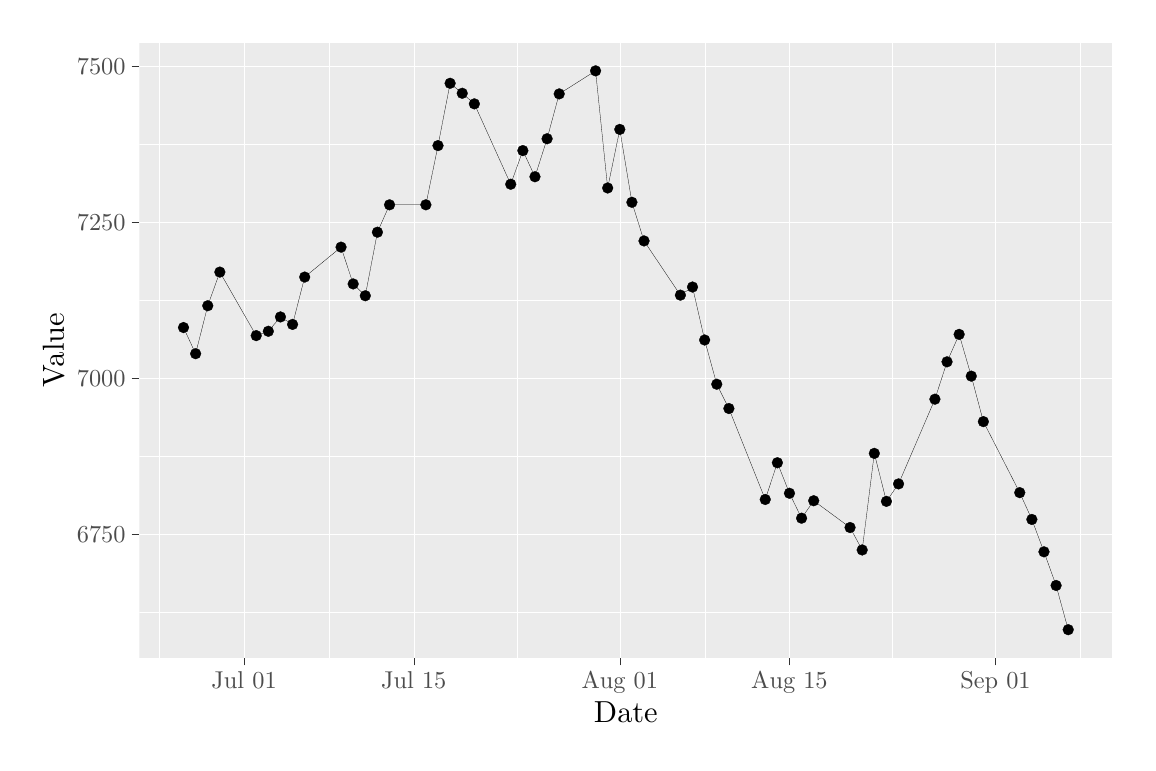
\begin{tikzpicture}[x=1pt,y=1pt]
\definecolor{fillColor}{RGB}{255,255,255}
\path[use as bounding box,fill=fillColor,fill opacity=0.00] (0,0) rectangle (397.48,258.37);
\begin{scope}
\path[clip] (  0.00,  0.00) rectangle (397.48,258.37);
\definecolor{drawColor}{RGB}{255,255,255}
\definecolor{fillColor}{RGB}{255,255,255}

\path[draw=drawColor,line width= 0.1pt,line join=round,line cap=round,fill=fillColor] (  0.00,  0.00) rectangle (397.48,258.37);
\end{scope}
\begin{scope}
\path[clip] ( 40.32, 30.73) rectangle (391.98,252.87);
\definecolor{fillColor}{gray}{0.92}

\path[fill=fillColor] ( 40.32, 30.73) rectangle (391.98,252.87);
\definecolor{drawColor}{RGB}{255,255,255}

\path[draw=drawColor,line width= 0.1pt,line join=round] ( 40.32, 47.35) --
	(391.98, 47.35);

\path[draw=drawColor,line width= 0.1pt,line join=round] ( 40.32,103.64) --
	(391.98,103.64);

\path[draw=drawColor,line width= 0.1pt,line join=round] ( 40.32,159.92) --
	(391.98,159.92);

\path[draw=drawColor,line width= 0.1pt,line join=round] ( 40.32,216.20) --
	(391.98,216.20);

\path[draw=drawColor,line width= 0.1pt,line join=round] ( 47.55, 30.73) --
	( 47.55,252.87);

\path[draw=drawColor,line width= 0.1pt,line join=round] (108.86, 30.73) --
	(108.86,252.87);

\path[draw=drawColor,line width= 0.1pt,line join=round] (176.74, 30.73) --
	(176.74,252.87);

\path[draw=drawColor,line width= 0.1pt,line join=round] (244.62, 30.73) --
	(244.62,252.87);

\path[draw=drawColor,line width= 0.1pt,line join=round] (312.50, 30.73) --
	(312.50,252.87);

\path[draw=drawColor,line width= 0.1pt,line join=round] (380.38, 30.73) --
	(380.38,252.87);

\path[draw=drawColor,line width= 0.1pt,line join=round] ( 40.32, 75.50) --
	(391.98, 75.50);

\path[draw=drawColor,line width= 0.1pt,line join=round] ( 40.32,131.78) --
	(391.98,131.78);

\path[draw=drawColor,line width= 0.1pt,line join=round] ( 40.32,188.06) --
	(391.98,188.06);

\path[draw=drawColor,line width= 0.1pt,line join=round] ( 40.32,244.34) --
	(391.98,244.34);

\path[draw=drawColor,line width= 0.1pt,line join=round] ( 78.20, 30.73) --
	( 78.20,252.87);

\path[draw=drawColor,line width= 0.1pt,line join=round] (139.51, 30.73) --
	(139.51,252.87);

\path[draw=drawColor,line width= 0.1pt,line join=round] (213.96, 30.73) --
	(213.96,252.87);

\path[draw=drawColor,line width= 0.1pt,line join=round] (275.27, 30.73) --
	(275.27,252.87);

\path[draw=drawColor,line width= 0.1pt,line join=round] (349.72, 30.73) --
	(349.72,252.87);
\definecolor{drawColor}{RGB}{0,0,0}

\path[draw=drawColor,line width= 0.1pt,line join=round] ( 56.31,150.01) --
	( 60.69,140.56) --
	( 65.07,157.89) --
	( 69.44,170.05) --
	( 82.58,147.09) --
	( 86.96,148.66) --
	( 91.34,153.84) --
	( 95.72,151.14) --
	(100.10,168.25) --
	(113.24,179.06) --
	(117.62,165.77) --
	(122.00,161.50) --
	(126.38,184.46) --
	(130.76,194.36) --
	(143.89,194.36) --
	(148.27,215.75) --
	(152.65,238.27) --
	(157.03,234.66) --
	(161.41,230.84) --
	(174.55,201.79) --
	(178.93,213.95) --
	(183.31,204.50) --
	(187.69,218.23) --
	(192.07,234.44) --
	(205.21,242.77) --
	(209.58,200.44) --
	(213.96,221.61) --
	(218.34,195.27) --
	(222.72,181.31) --
	(235.86,161.72) --
	(240.24,164.65) --
	(244.62,145.51) --
	(249.00,129.53) --
	(253.38,120.75) --
	(266.52, 87.88) --
	(270.90,101.16) --
	(275.27, 90.13) --
	(279.65, 81.12) --
	(284.03, 87.43) --
	(297.17, 77.75) --
	(301.55, 69.64) --
	(305.93,104.54) --
	(310.31, 87.20) --
	(314.69, 93.51) --
	(327.83,124.12) --
	(332.21,137.63) --
	(336.59,147.54) --
	(340.97,132.45) --
	(345.34,116.02) --
	(358.48, 90.35) --
	(362.86, 80.67) --
	(367.24, 68.97) --
	(371.62, 56.81) --
	(376.00, 40.83);
\definecolor{fillColor}{RGB}{0,0,0}

\path[draw=drawColor,line width= 0.1pt,line join=round,line cap=round,fill=fillColor] ( 56.31,150.01) circle (  1.96);

\path[draw=drawColor,line width= 0.1pt,line join=round,line cap=round,fill=fillColor] ( 60.69,140.56) circle (  1.96);

\path[draw=drawColor,line width= 0.1pt,line join=round,line cap=round,fill=fillColor] ( 65.07,157.89) circle (  1.96);

\path[draw=drawColor,line width= 0.1pt,line join=round,line cap=round,fill=fillColor] ( 69.44,170.05) circle (  1.96);

\path[draw=drawColor,line width= 0.1pt,line join=round,line cap=round,fill=fillColor] ( 82.58,147.09) circle (  1.96);

\path[draw=drawColor,line width= 0.1pt,line join=round,line cap=round,fill=fillColor] ( 86.96,148.66) circle (  1.96);

\path[draw=drawColor,line width= 0.1pt,line join=round,line cap=round,fill=fillColor] ( 91.34,153.84) circle (  1.96);

\path[draw=drawColor,line width= 0.1pt,line join=round,line cap=round,fill=fillColor] ( 95.72,151.14) circle (  1.96);

\path[draw=drawColor,line width= 0.1pt,line join=round,line cap=round,fill=fillColor] (100.10,168.25) circle (  1.96);

\path[draw=drawColor,line width= 0.1pt,line join=round,line cap=round,fill=fillColor] (113.24,179.06) circle (  1.96);

\path[draw=drawColor,line width= 0.1pt,line join=round,line cap=round,fill=fillColor] (117.62,165.77) circle (  1.96);

\path[draw=drawColor,line width= 0.1pt,line join=round,line cap=round,fill=fillColor] (122.00,161.50) circle (  1.96);

\path[draw=drawColor,line width= 0.1pt,line join=round,line cap=round,fill=fillColor] (126.38,184.46) circle (  1.96);

\path[draw=drawColor,line width= 0.1pt,line join=round,line cap=round,fill=fillColor] (130.76,194.36) circle (  1.96);

\path[draw=drawColor,line width= 0.1pt,line join=round,line cap=round,fill=fillColor] (143.89,194.36) circle (  1.96);

\path[draw=drawColor,line width= 0.1pt,line join=round,line cap=round,fill=fillColor] (148.27,215.75) circle (  1.96);

\path[draw=drawColor,line width= 0.1pt,line join=round,line cap=round,fill=fillColor] (152.65,238.27) circle (  1.96);

\path[draw=drawColor,line width= 0.1pt,line join=round,line cap=round,fill=fillColor] (157.03,234.66) circle (  1.96);

\path[draw=drawColor,line width= 0.1pt,line join=round,line cap=round,fill=fillColor] (161.41,230.84) circle (  1.96);

\path[draw=drawColor,line width= 0.1pt,line join=round,line cap=round,fill=fillColor] (174.55,201.79) circle (  1.96);

\path[draw=drawColor,line width= 0.1pt,line join=round,line cap=round,fill=fillColor] (178.93,213.95) circle (  1.96);

\path[draw=drawColor,line width= 0.1pt,line join=round,line cap=round,fill=fillColor] (183.31,204.50) circle (  1.96);

\path[draw=drawColor,line width= 0.1pt,line join=round,line cap=round,fill=fillColor] (187.69,218.23) circle (  1.96);

\path[draw=drawColor,line width= 0.1pt,line join=round,line cap=round,fill=fillColor] (192.07,234.44) circle (  1.96);

\path[draw=drawColor,line width= 0.1pt,line join=round,line cap=round,fill=fillColor] (205.21,242.77) circle (  1.96);

\path[draw=drawColor,line width= 0.1pt,line join=round,line cap=round,fill=fillColor] (209.58,200.44) circle (  1.96);

\path[draw=drawColor,line width= 0.1pt,line join=round,line cap=round,fill=fillColor] (213.96,221.61) circle (  1.96);

\path[draw=drawColor,line width= 0.1pt,line join=round,line cap=round,fill=fillColor] (218.34,195.27) circle (  1.96);

\path[draw=drawColor,line width= 0.1pt,line join=round,line cap=round,fill=fillColor] (222.72,181.31) circle (  1.96);

\path[draw=drawColor,line width= 0.1pt,line join=round,line cap=round,fill=fillColor] (235.86,161.72) circle (  1.96);

\path[draw=drawColor,line width= 0.1pt,line join=round,line cap=round,fill=fillColor] (240.24,164.65) circle (  1.96);

\path[draw=drawColor,line width= 0.1pt,line join=round,line cap=round,fill=fillColor] (244.62,145.51) circle (  1.96);

\path[draw=drawColor,line width= 0.1pt,line join=round,line cap=round,fill=fillColor] (249.00,129.53) circle (  1.96);

\path[draw=drawColor,line width= 0.1pt,line join=round,line cap=round,fill=fillColor] (253.38,120.75) circle (  1.96);

\path[draw=drawColor,line width= 0.1pt,line join=round,line cap=round,fill=fillColor] (266.52, 87.88) circle (  1.96);

\path[draw=drawColor,line width= 0.1pt,line join=round,line cap=round,fill=fillColor] (270.90,101.16) circle (  1.96);

\path[draw=drawColor,line width= 0.1pt,line join=round,line cap=round,fill=fillColor] (275.27, 90.13) circle (  1.96);

\path[draw=drawColor,line width= 0.1pt,line join=round,line cap=round,fill=fillColor] (279.65, 81.12) circle (  1.96);

\path[draw=drawColor,line width= 0.1pt,line join=round,line cap=round,fill=fillColor] (284.03, 87.43) circle (  1.96);

\path[draw=drawColor,line width= 0.1pt,line join=round,line cap=round,fill=fillColor] (297.17, 77.75) circle (  1.96);

\path[draw=drawColor,line width= 0.1pt,line join=round,line cap=round,fill=fillColor] (301.55, 69.64) circle (  1.96);

\path[draw=drawColor,line width= 0.1pt,line join=round,line cap=round,fill=fillColor] (305.93,104.54) circle (  1.96);

\path[draw=drawColor,line width= 0.1pt,line join=round,line cap=round,fill=fillColor] (310.31, 87.20) circle (  1.96);

\path[draw=drawColor,line width= 0.1pt,line join=round,line cap=round,fill=fillColor] (314.69, 93.51) circle (  1.96);

\path[draw=drawColor,line width= 0.1pt,line join=round,line cap=round,fill=fillColor] (327.83,124.12) circle (  1.96);

\path[draw=drawColor,line width= 0.1pt,line join=round,line cap=round,fill=fillColor] (332.21,137.63) circle (  1.96);

\path[draw=drawColor,line width= 0.1pt,line join=round,line cap=round,fill=fillColor] (336.59,147.54) circle (  1.96);

\path[draw=drawColor,line width= 0.1pt,line join=round,line cap=round,fill=fillColor] (340.97,132.45) circle (  1.96);

\path[draw=drawColor,line width= 0.1pt,line join=round,line cap=round,fill=fillColor] (345.34,116.02) circle (  1.96);

\path[draw=drawColor,line width= 0.1pt,line join=round,line cap=round,fill=fillColor] (358.48, 90.35) circle (  1.96);

\path[draw=drawColor,line width= 0.1pt,line join=round,line cap=round,fill=fillColor] (362.86, 80.67) circle (  1.96);

\path[draw=drawColor,line width= 0.1pt,line join=round,line cap=round,fill=fillColor] (367.24, 68.97) circle (  1.96);

\path[draw=drawColor,line width= 0.1pt,line join=round,line cap=round,fill=fillColor] (371.62, 56.81) circle (  1.96);

\path[draw=drawColor,line width= 0.1pt,line join=round,line cap=round,fill=fillColor] (376.00, 40.83) circle (  1.96);
\end{scope}
\begin{scope}
\path[clip] (  0.00,  0.00) rectangle (397.48,258.37);
\definecolor{drawColor}{gray}{0.30}

\node[text=drawColor,anchor=base east,inner sep=0pt, outer sep=0pt, scale=  0.88] at ( 35.37, 72.46) {6750};

\node[text=drawColor,anchor=base east,inner sep=0pt, outer sep=0pt, scale=  0.88] at ( 35.37,128.75) {7000};

\node[text=drawColor,anchor=base east,inner sep=0pt, outer sep=0pt, scale=  0.88] at ( 35.37,185.03) {7250};

\node[text=drawColor,anchor=base east,inner sep=0pt, outer sep=0pt, scale=  0.88] at ( 35.37,241.31) {7500};
\end{scope}
\begin{scope}
\path[clip] (  0.00,  0.00) rectangle (397.48,258.37);
\definecolor{drawColor}{gray}{0.20}

\path[draw=drawColor,line width= 0.1pt,line join=round] ( 37.57, 75.50) --
	( 40.32, 75.50);

\path[draw=drawColor,line width= 0.1pt,line join=round] ( 37.57,131.78) --
	( 40.32,131.78);

\path[draw=drawColor,line width= 0.1pt,line join=round] ( 37.57,188.06) --
	( 40.32,188.06);

\path[draw=drawColor,line width= 0.1pt,line join=round] ( 37.57,244.34) --
	( 40.32,244.34);
\end{scope}
\begin{scope}
\path[clip] (  0.00,  0.00) rectangle (397.48,258.37);
\definecolor{drawColor}{gray}{0.20}

\path[draw=drawColor,line width= 0.1pt,line join=round] ( 78.20, 27.98) --
	( 78.20, 30.73);

\path[draw=drawColor,line width= 0.1pt,line join=round] (139.51, 27.98) --
	(139.51, 30.73);

\path[draw=drawColor,line width= 0.1pt,line join=round] (213.96, 27.98) --
	(213.96, 30.73);

\path[draw=drawColor,line width= 0.1pt,line join=round] (275.27, 27.98) --
	(275.27, 30.73);

\path[draw=drawColor,line width= 0.1pt,line join=round] (349.72, 27.98) --
	(349.72, 30.73);
\end{scope}
\begin{scope}
\path[clip] (  0.00,  0.00) rectangle (397.48,258.37);
\definecolor{drawColor}{gray}{0.30}

\node[text=drawColor,anchor=base,inner sep=0pt, outer sep=0pt, scale=  0.88] at ( 78.20, 19.72) {Jul 01};

\node[text=drawColor,anchor=base,inner sep=0pt, outer sep=0pt, scale=  0.88] at (139.51, 19.72) {Jul 15};

\node[text=drawColor,anchor=base,inner sep=0pt, outer sep=0pt, scale=  0.88] at (213.96, 19.72) {Aug 01};

\node[text=drawColor,anchor=base,inner sep=0pt, outer sep=0pt, scale=  0.88] at (275.27, 19.72) {Aug 15};

\node[text=drawColor,anchor=base,inner sep=0pt, outer sep=0pt, scale=  0.88] at (349.72, 19.72) {Sep 01};
\end{scope}
\begin{scope}
\path[clip] (  0.00,  0.00) rectangle (397.48,258.37);
\definecolor{drawColor}{RGB}{0,0,0}

\node[text=drawColor,anchor=base,inner sep=0pt, outer sep=0pt, scale=  1.10] at (216.15,  7.44) {Date};
\end{scope}
\begin{scope}
\path[clip] (  0.00,  0.00) rectangle (397.48,258.37);
\definecolor{drawColor}{RGB}{0,0,0}

\node[text=drawColor,rotate= 90.00,anchor=base,inner sep=0pt, outer sep=0pt, scale=  1.10] at ( 13.08,141.80) {Value};
\end{scope}
\end{tikzpicture}

    
    \caption{Indices of Toyota within the evaluation time frame}
    \label{fig:analysis-indices-toyota}
\end{figure}   

\subsection{Volkswagen}
\label{ss:analysis-datasets-vw}

\begin{figure}[hbt]
    \centering
    % Created by tikzDevice version 0.12 on 2019-02-27 11:50:37
% !TEX encoding = UTF-8 Unicode
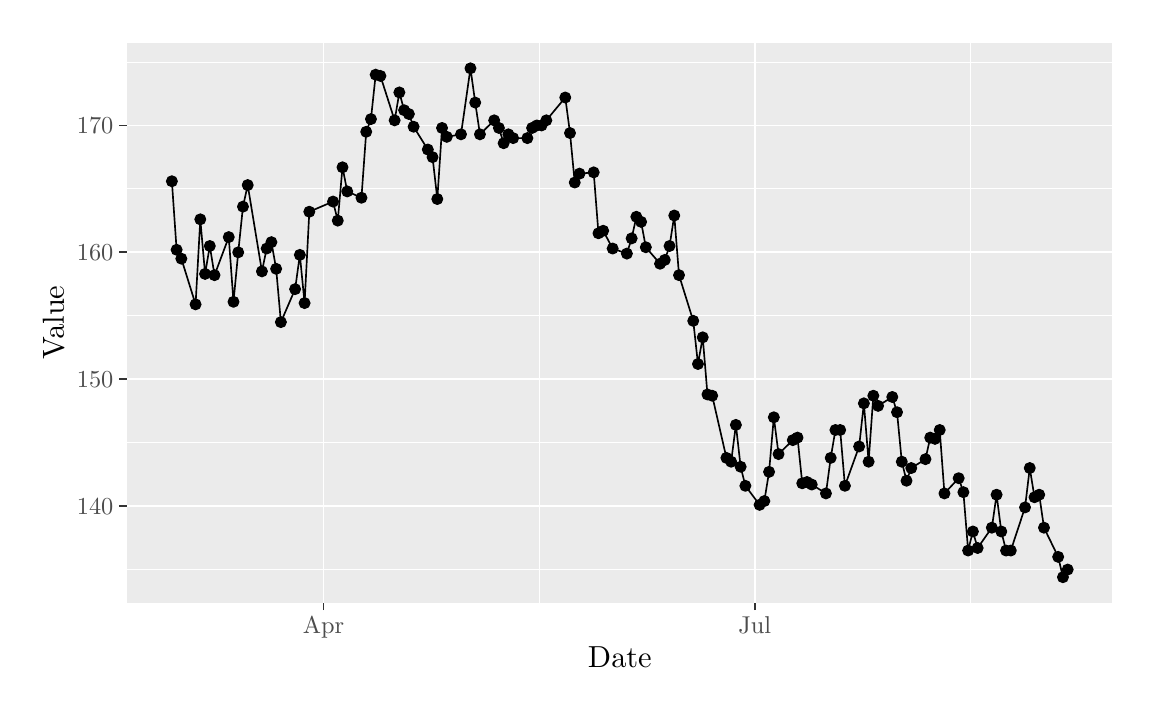
\begin{tikzpicture}[x=1pt,y=1pt]
\definecolor{fillColor}{RGB}{255,255,255}
\path[use as bounding box,fill=fillColor,fill opacity=0.00] (0,0) rectangle (397.48,238.49);
\begin{scope}
\path[clip] (  0.00,  0.00) rectangle (397.48,238.49);
\definecolor{drawColor}{RGB}{255,255,255}
\definecolor{fillColor}{RGB}{255,255,255}

\path[draw=drawColor,line width= 0.6pt,line join=round,line cap=round,fill=fillColor] (  0.00,  0.00) rectangle (397.48,238.49);
\end{scope}
\begin{scope}
\path[clip] ( 35.92, 30.73) rectangle (391.98,232.99);
\definecolor{fillColor}{gray}{0.92}

\path[fill=fillColor] ( 35.92, 30.73) rectangle (391.98,232.99);
\definecolor{drawColor}{RGB}{255,255,255}

\path[draw=drawColor,line width= 0.3pt,line join=round] ( 35.92, 42.67) --
	(391.98, 42.67);

\path[draw=drawColor,line width= 0.3pt,line join=round] ( 35.92, 88.53) --
	(391.98, 88.53);

\path[draw=drawColor,line width= 0.3pt,line join=round] ( 35.92,134.38) --
	(391.98,134.38);

\path[draw=drawColor,line width= 0.3pt,line join=round] ( 35.92,180.24) --
	(391.98,180.24);

\path[draw=drawColor,line width= 0.3pt,line join=round] ( 35.92,226.09) --
	(391.98,226.09);

\path[draw=drawColor,line width= 0.3pt,line join=round] (184.84, 30.73) --
	(184.84,232.99);

\path[draw=drawColor,line width= 0.3pt,line join=round] (340.69, 30.73) --
	(340.69,232.99);

\path[draw=drawColor,line width= 0.6pt,line join=round] ( 35.92, 65.60) --
	(391.98, 65.60);

\path[draw=drawColor,line width= 0.6pt,line join=round] ( 35.92,111.45) --
	(391.98,111.45);

\path[draw=drawColor,line width= 0.6pt,line join=round] ( 35.92,157.31) --
	(391.98,157.31);

\path[draw=drawColor,line width= 0.6pt,line join=round] ( 35.92,203.16) --
	(391.98,203.16);

\path[draw=drawColor,line width= 0.6pt,line join=round] (106.91, 30.73) --
	(106.91,232.99);

\path[draw=drawColor,line width= 0.6pt,line join=round] (262.76, 30.73) --
	(262.76,232.99);
\definecolor{drawColor}{RGB}{0,0,0}

\path[draw=drawColor,line width= 0.6pt,line join=round] ( 52.11,182.99) --
	( 53.82,158.23) --
	( 55.53,155.02) --
	( 60.67,138.51) --
	( 62.38,169.23) --
	( 64.10,149.51) --
	( 65.81,159.60) --
	( 67.52,149.06) --
	( 72.66,162.81) --
	( 74.37,139.43) --
	( 76.08,157.31) --
	( 77.80,173.82) --
	( 79.51,181.61) --
	( 84.65,150.43) --
	( 86.36,158.68) --
	( 88.07,160.98) --
	( 89.79,151.35) --
	( 91.50,132.09) --
	( 96.64,144.01) --
	( 98.35,156.39) --
	(100.06,138.97) --
	(101.77,171.98) --
	(110.34,175.65) --
	(112.05,168.77) --
	(113.76,188.03) --
	(115.48,179.32) --
	(120.61,177.03) --
	(122.33,200.87) --
	(124.04,205.46) --
	(125.75,221.50) --
	(127.46,221.05) --
	(132.60,205.00) --
	(134.31,215.09) --
	(136.03,208.67) --
	(137.74,207.29) --
	(139.45,202.70) --
	(144.59,194.45) --
	(146.30,191.70) --
	(148.02,176.57) --
	(149.73,202.25) --
	(151.44,199.04) --
	(156.58,199.95) --
	(160.00,223.80) --
	(161.72,211.42) --
	(163.43,199.95) --
	(168.57,205.00) --
	(170.28,202.25) --
	(171.99,196.74) --
	(173.71,199.95) --
	(175.42,198.58) --
	(180.56,198.58) --
	(182.27,202.25) --
	(183.98,203.16) --
	(185.69,203.16) --
	(187.41,205.00) --
	(194.26,213.25) --
	(195.97,200.41) --
	(197.68,182.53) --
	(199.40,185.74) --
	(204.53,186.20) --
	(206.25,164.19) --
	(207.96,165.10) --
	(211.38,158.68) --
	(216.52,156.85) --
	(218.24,162.35) --
	(219.95,170.15) --
	(221.66,168.31) --
	(223.37,159.14) --
	(228.51,153.18) --
	(230.22,154.56) --
	(231.94,159.60) --
	(233.65,170.61) --
	(235.36,149.06) --
	(240.50,132.55) --
	(242.21,116.96) --
	(243.93,126.59) --
	(245.64,105.95) --
	(247.35,105.49) --
	(252.49, 83.03) --
	(254.20, 81.65) --
	(255.91, 94.95) --
	(257.63, 79.82) --
	(259.34, 72.94) --
	(264.48, 66.06) --
	(266.19, 67.43) --
	(267.90, 77.98) --
	(269.62, 97.70) --
	(271.33, 84.40) --
	(276.47, 89.44) --
	(278.18, 90.36) --
	(279.89, 73.85) --
	(281.60, 74.31) --
	(283.32, 73.40) --
	(288.45, 70.19) --
	(290.17, 83.03) --
	(291.88, 93.11) --
	(293.59, 93.11) --
	(295.31, 72.94) --
	(300.44, 87.15) --
	(302.16,102.74) --
	(303.87, 81.65) --
	(305.58,105.49) --
	(307.29,101.83) --
	(312.43,105.04) --
	(314.14, 99.53) --
	(315.86, 81.65) --
	(317.57, 74.77) --
	(319.28, 79.36) --
	(324.42, 82.57) --
	(326.13, 90.36) --
	(327.85, 89.90) --
	(329.56, 93.11) --
	(331.27, 70.19) --
	(336.41, 75.69) --
	(338.12, 70.64) --
	(339.83, 49.55) --
	(341.55, 56.43) --
	(343.26, 50.47) --
	(348.40, 57.81) --
	(350.11, 69.73) --
	(351.82, 56.43) --
	(353.54, 49.55) --
	(355.25, 49.55) --
	(360.39, 65.14) --
	(362.10, 79.36) --
	(363.81, 68.81) --
	(365.52, 69.73) --
	(367.24, 57.81) --
	(372.37, 47.26) --
	(374.09, 39.92) --
	(375.80, 42.67);
\definecolor{fillColor}{RGB}{0,0,0}

\path[draw=drawColor,line width= 0.4pt,line join=round,line cap=round,fill=fillColor] ( 52.11,182.99) circle (  1.96);

\path[draw=drawColor,line width= 0.4pt,line join=round,line cap=round,fill=fillColor] ( 53.82,158.23) circle (  1.96);

\path[draw=drawColor,line width= 0.4pt,line join=round,line cap=round,fill=fillColor] ( 55.53,155.02) circle (  1.96);

\path[draw=drawColor,line width= 0.4pt,line join=round,line cap=round,fill=fillColor] ( 60.67,138.51) circle (  1.96);

\path[draw=drawColor,line width= 0.4pt,line join=round,line cap=round,fill=fillColor] ( 62.38,169.23) circle (  1.96);

\path[draw=drawColor,line width= 0.4pt,line join=round,line cap=round,fill=fillColor] ( 64.10,149.51) circle (  1.96);

\path[draw=drawColor,line width= 0.4pt,line join=round,line cap=round,fill=fillColor] ( 65.81,159.60) circle (  1.96);

\path[draw=drawColor,line width= 0.4pt,line join=round,line cap=round,fill=fillColor] ( 67.52,149.06) circle (  1.96);

\path[draw=drawColor,line width= 0.4pt,line join=round,line cap=round,fill=fillColor] ( 72.66,162.81) circle (  1.96);

\path[draw=drawColor,line width= 0.4pt,line join=round,line cap=round,fill=fillColor] ( 74.37,139.43) circle (  1.96);

\path[draw=drawColor,line width= 0.4pt,line join=round,line cap=round,fill=fillColor] ( 76.08,157.31) circle (  1.96);

\path[draw=drawColor,line width= 0.4pt,line join=round,line cap=round,fill=fillColor] ( 77.80,173.82) circle (  1.96);

\path[draw=drawColor,line width= 0.4pt,line join=round,line cap=round,fill=fillColor] ( 79.51,181.61) circle (  1.96);

\path[draw=drawColor,line width= 0.4pt,line join=round,line cap=round,fill=fillColor] ( 84.65,150.43) circle (  1.96);

\path[draw=drawColor,line width= 0.4pt,line join=round,line cap=round,fill=fillColor] ( 86.36,158.68) circle (  1.96);

\path[draw=drawColor,line width= 0.4pt,line join=round,line cap=round,fill=fillColor] ( 88.07,160.98) circle (  1.96);

\path[draw=drawColor,line width= 0.4pt,line join=round,line cap=round,fill=fillColor] ( 89.79,151.35) circle (  1.96);

\path[draw=drawColor,line width= 0.4pt,line join=round,line cap=round,fill=fillColor] ( 91.50,132.09) circle (  1.96);

\path[draw=drawColor,line width= 0.4pt,line join=round,line cap=round,fill=fillColor] ( 96.64,144.01) circle (  1.96);

\path[draw=drawColor,line width= 0.4pt,line join=round,line cap=round,fill=fillColor] ( 98.35,156.39) circle (  1.96);

\path[draw=drawColor,line width= 0.4pt,line join=round,line cap=round,fill=fillColor] (100.06,138.97) circle (  1.96);

\path[draw=drawColor,line width= 0.4pt,line join=round,line cap=round,fill=fillColor] (101.77,171.98) circle (  1.96);

\path[draw=drawColor,line width= 0.4pt,line join=round,line cap=round,fill=fillColor] (110.34,175.65) circle (  1.96);

\path[draw=drawColor,line width= 0.4pt,line join=round,line cap=round,fill=fillColor] (112.05,168.77) circle (  1.96);

\path[draw=drawColor,line width= 0.4pt,line join=round,line cap=round,fill=fillColor] (113.76,188.03) circle (  1.96);

\path[draw=drawColor,line width= 0.4pt,line join=round,line cap=round,fill=fillColor] (115.48,179.32) circle (  1.96);

\path[draw=drawColor,line width= 0.4pt,line join=round,line cap=round,fill=fillColor] (120.61,177.03) circle (  1.96);

\path[draw=drawColor,line width= 0.4pt,line join=round,line cap=round,fill=fillColor] (122.33,200.87) circle (  1.96);

\path[draw=drawColor,line width= 0.4pt,line join=round,line cap=round,fill=fillColor] (124.04,205.46) circle (  1.96);

\path[draw=drawColor,line width= 0.4pt,line join=round,line cap=round,fill=fillColor] (125.75,221.50) circle (  1.96);

\path[draw=drawColor,line width= 0.4pt,line join=round,line cap=round,fill=fillColor] (127.46,221.05) circle (  1.96);

\path[draw=drawColor,line width= 0.4pt,line join=round,line cap=round,fill=fillColor] (132.60,205.00) circle (  1.96);

\path[draw=drawColor,line width= 0.4pt,line join=round,line cap=round,fill=fillColor] (134.31,215.09) circle (  1.96);

\path[draw=drawColor,line width= 0.4pt,line join=round,line cap=round,fill=fillColor] (136.03,208.67) circle (  1.96);

\path[draw=drawColor,line width= 0.4pt,line join=round,line cap=round,fill=fillColor] (137.74,207.29) circle (  1.96);

\path[draw=drawColor,line width= 0.4pt,line join=round,line cap=round,fill=fillColor] (139.45,202.70) circle (  1.96);

\path[draw=drawColor,line width= 0.4pt,line join=round,line cap=round,fill=fillColor] (144.59,194.45) circle (  1.96);

\path[draw=drawColor,line width= 0.4pt,line join=round,line cap=round,fill=fillColor] (146.30,191.70) circle (  1.96);

\path[draw=drawColor,line width= 0.4pt,line join=round,line cap=round,fill=fillColor] (148.02,176.57) circle (  1.96);

\path[draw=drawColor,line width= 0.4pt,line join=round,line cap=round,fill=fillColor] (149.73,202.25) circle (  1.96);

\path[draw=drawColor,line width= 0.4pt,line join=round,line cap=round,fill=fillColor] (151.44,199.04) circle (  1.96);

\path[draw=drawColor,line width= 0.4pt,line join=round,line cap=round,fill=fillColor] (156.58,199.95) circle (  1.96);

\path[draw=drawColor,line width= 0.4pt,line join=round,line cap=round,fill=fillColor] (160.00,223.80) circle (  1.96);

\path[draw=drawColor,line width= 0.4pt,line join=round,line cap=round,fill=fillColor] (161.72,211.42) circle (  1.96);

\path[draw=drawColor,line width= 0.4pt,line join=round,line cap=round,fill=fillColor] (163.43,199.95) circle (  1.96);

\path[draw=drawColor,line width= 0.4pt,line join=round,line cap=round,fill=fillColor] (168.57,205.00) circle (  1.96);

\path[draw=drawColor,line width= 0.4pt,line join=round,line cap=round,fill=fillColor] (170.28,202.25) circle (  1.96);

\path[draw=drawColor,line width= 0.4pt,line join=round,line cap=round,fill=fillColor] (171.99,196.74) circle (  1.96);

\path[draw=drawColor,line width= 0.4pt,line join=round,line cap=round,fill=fillColor] (173.71,199.95) circle (  1.96);

\path[draw=drawColor,line width= 0.4pt,line join=round,line cap=round,fill=fillColor] (175.42,198.58) circle (  1.96);

\path[draw=drawColor,line width= 0.4pt,line join=round,line cap=round,fill=fillColor] (180.56,198.58) circle (  1.96);

\path[draw=drawColor,line width= 0.4pt,line join=round,line cap=round,fill=fillColor] (182.27,202.25) circle (  1.96);

\path[draw=drawColor,line width= 0.4pt,line join=round,line cap=round,fill=fillColor] (183.98,203.16) circle (  1.96);

\path[draw=drawColor,line width= 0.4pt,line join=round,line cap=round,fill=fillColor] (185.69,203.16) circle (  1.96);

\path[draw=drawColor,line width= 0.4pt,line join=round,line cap=round,fill=fillColor] (187.41,205.00) circle (  1.96);

\path[draw=drawColor,line width= 0.4pt,line join=round,line cap=round,fill=fillColor] (194.26,213.25) circle (  1.96);

\path[draw=drawColor,line width= 0.4pt,line join=round,line cap=round,fill=fillColor] (195.97,200.41) circle (  1.96);

\path[draw=drawColor,line width= 0.4pt,line join=round,line cap=round,fill=fillColor] (197.68,182.53) circle (  1.96);

\path[draw=drawColor,line width= 0.4pt,line join=round,line cap=round,fill=fillColor] (199.40,185.74) circle (  1.96);

\path[draw=drawColor,line width= 0.4pt,line join=round,line cap=round,fill=fillColor] (204.53,186.20) circle (  1.96);

\path[draw=drawColor,line width= 0.4pt,line join=round,line cap=round,fill=fillColor] (206.25,164.19) circle (  1.96);

\path[draw=drawColor,line width= 0.4pt,line join=round,line cap=round,fill=fillColor] (207.96,165.10) circle (  1.96);

\path[draw=drawColor,line width= 0.4pt,line join=round,line cap=round,fill=fillColor] (211.38,158.68) circle (  1.96);

\path[draw=drawColor,line width= 0.4pt,line join=round,line cap=round,fill=fillColor] (216.52,156.85) circle (  1.96);

\path[draw=drawColor,line width= 0.4pt,line join=round,line cap=round,fill=fillColor] (218.24,162.35) circle (  1.96);

\path[draw=drawColor,line width= 0.4pt,line join=round,line cap=round,fill=fillColor] (219.95,170.15) circle (  1.96);

\path[draw=drawColor,line width= 0.4pt,line join=round,line cap=round,fill=fillColor] (221.66,168.31) circle (  1.96);

\path[draw=drawColor,line width= 0.4pt,line join=round,line cap=round,fill=fillColor] (223.37,159.14) circle (  1.96);

\path[draw=drawColor,line width= 0.4pt,line join=round,line cap=round,fill=fillColor] (228.51,153.18) circle (  1.96);

\path[draw=drawColor,line width= 0.4pt,line join=round,line cap=round,fill=fillColor] (230.22,154.56) circle (  1.96);

\path[draw=drawColor,line width= 0.4pt,line join=round,line cap=round,fill=fillColor] (231.94,159.60) circle (  1.96);

\path[draw=drawColor,line width= 0.4pt,line join=round,line cap=round,fill=fillColor] (233.65,170.61) circle (  1.96);

\path[draw=drawColor,line width= 0.4pt,line join=round,line cap=round,fill=fillColor] (235.36,149.06) circle (  1.96);

\path[draw=drawColor,line width= 0.4pt,line join=round,line cap=round,fill=fillColor] (240.50,132.55) circle (  1.96);

\path[draw=drawColor,line width= 0.4pt,line join=round,line cap=round,fill=fillColor] (242.21,116.96) circle (  1.96);

\path[draw=drawColor,line width= 0.4pt,line join=round,line cap=round,fill=fillColor] (243.93,126.59) circle (  1.96);

\path[draw=drawColor,line width= 0.4pt,line join=round,line cap=round,fill=fillColor] (245.64,105.95) circle (  1.96);

\path[draw=drawColor,line width= 0.4pt,line join=round,line cap=round,fill=fillColor] (247.35,105.49) circle (  1.96);

\path[draw=drawColor,line width= 0.4pt,line join=round,line cap=round,fill=fillColor] (252.49, 83.03) circle (  1.96);

\path[draw=drawColor,line width= 0.4pt,line join=round,line cap=round,fill=fillColor] (254.20, 81.65) circle (  1.96);

\path[draw=drawColor,line width= 0.4pt,line join=round,line cap=round,fill=fillColor] (255.91, 94.95) circle (  1.96);

\path[draw=drawColor,line width= 0.4pt,line join=round,line cap=round,fill=fillColor] (257.63, 79.82) circle (  1.96);

\path[draw=drawColor,line width= 0.4pt,line join=round,line cap=round,fill=fillColor] (259.34, 72.94) circle (  1.96);

\path[draw=drawColor,line width= 0.4pt,line join=round,line cap=round,fill=fillColor] (264.48, 66.06) circle (  1.96);

\path[draw=drawColor,line width= 0.4pt,line join=round,line cap=round,fill=fillColor] (266.19, 67.43) circle (  1.96);

\path[draw=drawColor,line width= 0.4pt,line join=round,line cap=round,fill=fillColor] (267.90, 77.98) circle (  1.96);

\path[draw=drawColor,line width= 0.4pt,line join=round,line cap=round,fill=fillColor] (269.62, 97.70) circle (  1.96);

\path[draw=drawColor,line width= 0.4pt,line join=round,line cap=round,fill=fillColor] (271.33, 84.40) circle (  1.96);

\path[draw=drawColor,line width= 0.4pt,line join=round,line cap=round,fill=fillColor] (276.47, 89.44) circle (  1.96);

\path[draw=drawColor,line width= 0.4pt,line join=round,line cap=round,fill=fillColor] (278.18, 90.36) circle (  1.96);

\path[draw=drawColor,line width= 0.4pt,line join=round,line cap=round,fill=fillColor] (279.89, 73.85) circle (  1.96);

\path[draw=drawColor,line width= 0.4pt,line join=round,line cap=round,fill=fillColor] (281.60, 74.31) circle (  1.96);

\path[draw=drawColor,line width= 0.4pt,line join=round,line cap=round,fill=fillColor] (283.32, 73.40) circle (  1.96);

\path[draw=drawColor,line width= 0.4pt,line join=round,line cap=round,fill=fillColor] (288.45, 70.19) circle (  1.96);

\path[draw=drawColor,line width= 0.4pt,line join=round,line cap=round,fill=fillColor] (290.17, 83.03) circle (  1.96);

\path[draw=drawColor,line width= 0.4pt,line join=round,line cap=round,fill=fillColor] (291.88, 93.11) circle (  1.96);

\path[draw=drawColor,line width= 0.4pt,line join=round,line cap=round,fill=fillColor] (293.59, 93.11) circle (  1.96);

\path[draw=drawColor,line width= 0.4pt,line join=round,line cap=round,fill=fillColor] (295.31, 72.94) circle (  1.96);

\path[draw=drawColor,line width= 0.4pt,line join=round,line cap=round,fill=fillColor] (300.44, 87.15) circle (  1.96);

\path[draw=drawColor,line width= 0.4pt,line join=round,line cap=round,fill=fillColor] (302.16,102.74) circle (  1.96);

\path[draw=drawColor,line width= 0.4pt,line join=round,line cap=round,fill=fillColor] (303.87, 81.65) circle (  1.96);

\path[draw=drawColor,line width= 0.4pt,line join=round,line cap=round,fill=fillColor] (305.58,105.49) circle (  1.96);

\path[draw=drawColor,line width= 0.4pt,line join=round,line cap=round,fill=fillColor] (307.29,101.83) circle (  1.96);

\path[draw=drawColor,line width= 0.4pt,line join=round,line cap=round,fill=fillColor] (312.43,105.04) circle (  1.96);

\path[draw=drawColor,line width= 0.4pt,line join=round,line cap=round,fill=fillColor] (314.14, 99.53) circle (  1.96);

\path[draw=drawColor,line width= 0.4pt,line join=round,line cap=round,fill=fillColor] (315.86, 81.65) circle (  1.96);

\path[draw=drawColor,line width= 0.4pt,line join=round,line cap=round,fill=fillColor] (317.57, 74.77) circle (  1.96);

\path[draw=drawColor,line width= 0.4pt,line join=round,line cap=round,fill=fillColor] (319.28, 79.36) circle (  1.96);

\path[draw=drawColor,line width= 0.4pt,line join=round,line cap=round,fill=fillColor] (324.42, 82.57) circle (  1.96);

\path[draw=drawColor,line width= 0.4pt,line join=round,line cap=round,fill=fillColor] (326.13, 90.36) circle (  1.96);

\path[draw=drawColor,line width= 0.4pt,line join=round,line cap=round,fill=fillColor] (327.85, 89.90) circle (  1.96);

\path[draw=drawColor,line width= 0.4pt,line join=round,line cap=round,fill=fillColor] (329.56, 93.11) circle (  1.96);

\path[draw=drawColor,line width= 0.4pt,line join=round,line cap=round,fill=fillColor] (331.27, 70.19) circle (  1.96);

\path[draw=drawColor,line width= 0.4pt,line join=round,line cap=round,fill=fillColor] (336.41, 75.69) circle (  1.96);

\path[draw=drawColor,line width= 0.4pt,line join=round,line cap=round,fill=fillColor] (338.12, 70.64) circle (  1.96);

\path[draw=drawColor,line width= 0.4pt,line join=round,line cap=round,fill=fillColor] (339.83, 49.55) circle (  1.96);

\path[draw=drawColor,line width= 0.4pt,line join=round,line cap=round,fill=fillColor] (341.55, 56.43) circle (  1.96);

\path[draw=drawColor,line width= 0.4pt,line join=round,line cap=round,fill=fillColor] (343.26, 50.47) circle (  1.96);

\path[draw=drawColor,line width= 0.4pt,line join=round,line cap=round,fill=fillColor] (348.40, 57.81) circle (  1.96);

\path[draw=drawColor,line width= 0.4pt,line join=round,line cap=round,fill=fillColor] (350.11, 69.73) circle (  1.96);

\path[draw=drawColor,line width= 0.4pt,line join=round,line cap=round,fill=fillColor] (351.82, 56.43) circle (  1.96);

\path[draw=drawColor,line width= 0.4pt,line join=round,line cap=round,fill=fillColor] (353.54, 49.55) circle (  1.96);

\path[draw=drawColor,line width= 0.4pt,line join=round,line cap=round,fill=fillColor] (355.25, 49.55) circle (  1.96);

\path[draw=drawColor,line width= 0.4pt,line join=round,line cap=round,fill=fillColor] (360.39, 65.14) circle (  1.96);

\path[draw=drawColor,line width= 0.4pt,line join=round,line cap=round,fill=fillColor] (362.10, 79.36) circle (  1.96);

\path[draw=drawColor,line width= 0.4pt,line join=round,line cap=round,fill=fillColor] (363.81, 68.81) circle (  1.96);

\path[draw=drawColor,line width= 0.4pt,line join=round,line cap=round,fill=fillColor] (365.52, 69.73) circle (  1.96);

\path[draw=drawColor,line width= 0.4pt,line join=round,line cap=round,fill=fillColor] (367.24, 57.81) circle (  1.96);

\path[draw=drawColor,line width= 0.4pt,line join=round,line cap=round,fill=fillColor] (372.37, 47.26) circle (  1.96);

\path[draw=drawColor,line width= 0.4pt,line join=round,line cap=round,fill=fillColor] (374.09, 39.92) circle (  1.96);

\path[draw=drawColor,line width= 0.4pt,line join=round,line cap=round,fill=fillColor] (375.80, 42.67) circle (  1.96);
\end{scope}
\begin{scope}
\path[clip] (  0.00,  0.00) rectangle (397.48,238.49);
\definecolor{drawColor}{gray}{0.30}

\node[text=drawColor,anchor=base east,inner sep=0pt, outer sep=0pt, scale=  0.88] at ( 30.97, 62.57) {140};

\node[text=drawColor,anchor=base east,inner sep=0pt, outer sep=0pt, scale=  0.88] at ( 30.97,108.42) {150};

\node[text=drawColor,anchor=base east,inner sep=0pt, outer sep=0pt, scale=  0.88] at ( 30.97,154.28) {160};

\node[text=drawColor,anchor=base east,inner sep=0pt, outer sep=0pt, scale=  0.88] at ( 30.97,200.13) {170};
\end{scope}
\begin{scope}
\path[clip] (  0.00,  0.00) rectangle (397.48,238.49);
\definecolor{drawColor}{gray}{0.20}

\path[draw=drawColor,line width= 0.6pt,line join=round] ( 33.17, 65.60) --
	( 35.92, 65.60);

\path[draw=drawColor,line width= 0.6pt,line join=round] ( 33.17,111.45) --
	( 35.92,111.45);

\path[draw=drawColor,line width= 0.6pt,line join=round] ( 33.17,157.31) --
	( 35.92,157.31);

\path[draw=drawColor,line width= 0.6pt,line join=round] ( 33.17,203.16) --
	( 35.92,203.16);
\end{scope}
\begin{scope}
\path[clip] (  0.00,  0.00) rectangle (397.48,238.49);
\definecolor{drawColor}{gray}{0.20}

\path[draw=drawColor,line width= 0.6pt,line join=round] (106.91, 27.98) --
	(106.91, 30.73);

\path[draw=drawColor,line width= 0.6pt,line join=round] (262.76, 27.98) --
	(262.76, 30.73);
\end{scope}
\begin{scope}
\path[clip] (  0.00,  0.00) rectangle (397.48,238.49);
\definecolor{drawColor}{gray}{0.30}

\node[text=drawColor,anchor=base,inner sep=0pt, outer sep=0pt, scale=  0.88] at (106.91, 19.72) {Apr};

\node[text=drawColor,anchor=base,inner sep=0pt, outer sep=0pt, scale=  0.88] at (262.76, 19.72) {Jul};
\end{scope}
\begin{scope}
\path[clip] (  0.00,  0.00) rectangle (397.48,238.49);
\definecolor{drawColor}{RGB}{0,0,0}

\node[text=drawColor,anchor=base,inner sep=0pt, outer sep=0pt, scale=  1.10] at (213.95,  7.44) {Date};
\end{scope}
\begin{scope}
\path[clip] (  0.00,  0.00) rectangle (397.48,238.49);
\definecolor{drawColor}{RGB}{0,0,0}

\node[text=drawColor,rotate= 90.00,anchor=base,inner sep=0pt, outer sep=0pt, scale=  1.10] at ( 13.08,131.86) {Value};
\end{scope}
\end{tikzpicture}

    
    \caption{Indices of VW within the evaluation time frame}
    \label{fig:analysis-indices-vw}
\end{figure}   

\section{Hyper-parameters}
\label{s:analysis-pipelines}
% best estimator pipeline

\section{Sentiment Time Series}
\label{s:analysis-sentiments}
% depict time series

\section{Comparison of Time Series}
\label{s:analysis-granger}
% granger causality

